% future/tm.tex
% mainfile: ../perfbook.tex
% SPDX-License-Identifier: CC-BY-SA-3.0

\section{Transactional Memory}
\label{sec:future:Transactional Memory}
\epigraph{Everything should be as simple as it can be, but not simpler.}
	 {\emph{Albert Einstein, by way of Louis Zukofsky}}

데이터베이스 외 영역에서 트랜잭션을 사용하려는 아이디어는 수십년 전부터
시작되었는데~\cite{DBLomet1977SIGSOFT,Knight:1986:AMF:319838.319854,Herlihy93a},
데이터베이스와 비 데이터베이스 트랜잭션 사이의 중요 차이점은 비 데이터베이스
트랜잭션은 데이터베이스 트랜잭션을 정의하는 속성인 ``ACID''\footnote{
	Atomicity (원자성), consistency (일관성), isolation (격리), 그리고
	durability (지속성).}
중 ``D'' 를 제거한다는 겁니다.
메모리 기반 트랜잭션, 또는 ``transactional memory (트랜잭셔널 메모리)'' (TM) 을
지원한다는 아이디어는 하드웨어에서는 비교적 최근의 일이나~\cite{Herlihy93a},
불행히도 일반 상용 하드웨어에서 그런 트랜잭션을 지원하는건 비슷한 다른 제안들은
진행되었음에도~\cite{JMStone93} 곧바로 진행되지 않았습니다.
그리 오래지 않아, Shavit 과 Touitou 는 일반 상용 하드웨어에서 돌릴 수 있으며
메모리 순서 문제를 주거나 받을 수 있는~\cite{Shavit95} 트랜잭셔널 메모리의
소프트웨어 구현 (STM) 을 제안했습니다.
이 제안은 여러 해동안 차차 시들어갔는데, 아마도 연구자 커뮤니티의 관심은
non-blocking 동기화에 흡수되었기 때문일 겁니다 (\cref{sec:advsync:Non-Blocking
Synchronization} 를 참고하세요).

\iffalse

The idea of using transactions outside of databases goes back many
decades~\cite{DBLomet1977SIGSOFT,Knight:1986:AMF:319838.319854,Herlihy93a},
with the key difference between
database and non-database transactions being that non-database transactions
drop the ``D'' in the ``ACID''\footnote{
	Atomicity, consistency, isolation, and durability.}
properties defining database transactions.
The idea of supporting memory-based transactions, or ``transactional memory''
(TM), in hardware
is more recent~\cite{Herlihy93a}, but unfortunately, support for such
transactions in commodity hardware was not immediately forthcoming,
despite other somewhat similar proposals being put forward~\cite{JMStone93}.
Not long after, Shavit and Touitou proposed a software-only implementation
of transactional memory (STM) that was capable of running on commodity
hardware, give or take memory-ordering issues~\cite{Shavit95}.
This proposal languished for many years, perhaps due to the fact that
the research community's attention was absorbed by non-blocking
synchronization (see \cref{sec:advsync:Non-Blocking Synchronization}).

\fi

하지만 세기가 바뀌며, TM 은 더 많은 관심을 받기
시작했으며~\cite{Martinez01a,Rajwar01a}, 그 십년의 중반에 이르러서는 관심의
정도가 ``작열했다''~\cite{MauriceHerlihy2005-TM-manifesto.pldi,
DanGrossman2007TMGCAnalogy} 고 말할 수 있으며, 약간의 경고 목소리만
존재했습니다~\cite{Blundell2005DebunkTM,McKenney2007PLOSTM}.

\iffalse

But by the turn of the century, TM started receiving
more attention~\cite{Martinez01a,Rajwar01a}, and by the middle of the
decade, the level of interest can only be termed
``incandescent''~\cite{MauriceHerlihy2005-TM-manifesto.pldi,
DanGrossman2007TMGCAnalogy}, with only a few voices of
caution~\cite{Blundell2005DebunkTM,McKenney2007PLOSTM}.

\fi

TM 의 기본 아이디어는 코드의 일부를 원자적으로 수행하여 다른 쓰레드는 중간
상태를 볼 수 없게 하자는 겁니다.
보통 그렇듯, TM 의 의미 규칙은 상당한 성능과 확장성 하락을 초래할 수 있지만 각
트랜잭션을 회귀적으로 획득될 수 있는 전역 락 획득과 해제로 대체될 수 있습니다.
하드웨어든 소프트웨어든 TM 구현에서 피할 수 없는 복잡도의 대부분은 동시의
트랜잭션이 안전하게 병렬로 수행될 수 있을 때 효율적으로 파악될 수 있습니다.
이 파악은 동적으로 이루어지므로, 충돌하는 트랜잭션은 취소되거나 ``롤백 (rolled
back)'' 될 수 있으며, 일부 구현에서는 이 실패 모드가 프로그래머에게 보여집니다.

\iffalse

The basic idea behind TM is to execute a section of
code atomically, so that other threads see no intermediate state.
As such, the semantics of TM could be implemented
by simply replacing each transaction with a recursively acquirable
global lock acquisition and release, albeit with abysmal performance
and scalability.
Much of the complexity inherent in TM implementations, whether hardware
or software, is efficiently detecting when concurrent transactions can safely
run in parallel.
Because this detection is done dynamically, conflicting transactions
can be aborted or ``rolled back'', and in some implementations, this
failure mode is visible to the programmer.

\fi

트랜잭션 롤백은 트랜잭션 크기가 작아질수록 더욱 이뤄지기 어려우므로, 스택, 큐,
해쉬 테이블, 그리고 탐색 트리에서 사용되는 링크드 리스트 조정 같은 작은 메모리
기반 오퍼레이션에 상당히 매력적일 겁니다.
그러나, 특히 I/O 와 프로세스 생성과 같은 비 메모리 오퍼레이션을 포함하는 큰
트랜잭션을 위한 경우는 현재로썬 훨씬 어렵습니다.
다음 섹션들은 ``어디에나 트랜잭셔널
메모리를''~\cite{PaulEMcKenney2009TMeverywhere} 이라는 큰 비전에의 현재의
문제들을 알아봅니다.
\Cref{sec:future:Outside World} 는 외부의 세계와 상호작용하는 과정에서 부딪히는
문제들을 알아보고,
\cref{sec:future:Process Modification} 는 프로세스 수정 기능들과의 상호작용을
알아보며,
\cref{sec:future:Synchronization} 는 다른 동기화 기능들과의 상호작용을
알아보고, 마지막으로
\cref{sec:future:Discussion} 는 일부 토론과 함께 장을 닫습니다.

\iffalse

Because transaction roll-back is increasingly unlikely as transaction
size decreases, TM might become quite attractive for small memory-based
operations,
such as linked-list manipulations used for stacks, queues, hash tables,
and search trees.
However, it is currently much more difficult to make the case for large
transactions, particularly those containing non-memory operations such
as I/O and process creation.
The following sections look at current challenges to the grand vision of
``Transactional Memory Everywhere''~\cite{PaulEMcKenney2009TMeverywhere}.
\Cref{sec:future:Outside World} examines the challenges faced
interacting with the outside world,
\cref{sec:future:Process Modification} looks at interactions
with process modification primitives,
\cref{sec:future:Synchronization} explores interactions with
other synchronization primitives, and finally
\cref{sec:future:Discussion} closes with some discussion.

\fi

\subsection{Outside World}
\label{sec:future:Outside World}

\ppl{Donald}{Knuth} 의 현명한 말을 빌리자면:

\iffalse

In the wise words of \ppl{Donald}{Knuth}:

\fi

\begin{quote}
	많은 컴퓨터 사용자들이 입출력이 ``진짜 프로그래밍'' 의 실제 부분이
	아니라 기계 안팎에서 정보를 얻기 위해 (불행히도) 이루어져야만 하는 것일
	뿐이라고 느낍니다.

	\iffalse

	Many computer users feel that input and output are not actually part
	of ``real programming,'' they are merely things that (unfortunately)
	must be done in order to get information in and out of the machine.

	\fi

\end{quote}

우리가 이 입출력을 ``진짜 프로그래밍'' 이라고 믿든 안믿든, 사실은 대부분의
컴퓨터 시스템에서 외부와의 상호작용은 첫번째 요구사항이라는 겁니다.
따라서 이 섹션은 트랜잭셔널 메모리의 I/O 오퍼레이션, 시간 지연, 또는 영구
저장장치를 통해서 이루어질 수 있는 그런 상호 작용 능력을 비평해 봅니다.

\iffalse

Whether we believe that input and output are ``real programming'' or
not, the fact is that for most computer systems, interaction with the
outside world is a first-class requirement.
This section therefore critiques transactional memory's ability to
so interact, whether via I/O operations, time delays, or persistent
storage.

\fi

\subsubsection{I/O Operations}
\label{sec:future:I/O Operations}

우린 I/O 오퍼레이션을 필요하다면 락 기반 크리티컬 섹션 내에서 해저드 포인터를
잡은 채, 시퀀스 락킹 read-side 크리티컬 섹션에서, 또는 userspace-RCU read-side
크리티컬 섹션에서, 그리고 심지어는 이 모든 것을 한꺼번에 한 채로 수행할 수
있습니다.
여러분이 I/O 오퍼레이션을 트랜잭션 형태로 수행하려 하면 어떤 일이 벌어질까요?

여기서의 문제는 트랜잭션은 예를 들면 충돌 때문에 롤백될 수 있다는 겁니다.
대략적으로 말하자면, 이는 해당 트랜잭션 내의 모든 오퍼레이션이 취소 가능해서 이
오퍼레이션을 두번 수행하는 것이 한번 수행되었을 때와 같은 효과를 내야 할 것을
필요로 합니다.
불행히도, I/O 는 일반적으로 취소 불가한 오퍼레이션의 원형이어서, 트랜잭션 내에
일반 I/O 오퍼레이션을 포함하기 어렵게 합니다.
실제로, 일반 I/O 는 취소 불가합니다:
일단 핵전쟁을 시작하는 버튼을 누르고 나면, 되돌릴 수 없습니다.

여기 트랜잭션 내에서 I/O 를 처리하기 위한 일부 선택사항이 있습니다:

\iffalse

One can execute I/O operations within a lock-based critical section,
while holding a hazard pointer, within a sequence-locking read-side
critical section, and from within a userspace-RCU read-side critical
section, and even all at the same time, if need be.
What happens when you attempt to execute an I/O operation from within
a transaction?

The underlying problem is that transactions may be rolled back, for
example, due to conflicts.
Roughly speaking, this requires that all operations within any given
transaction be revocable, so that executing the operation twice has
the same effect as executing it once.
Unfortunately, I/O is in general the prototypical irrevocable
operation, making it difficult to include general I/O operations in
transactions.
In fact, general I/O is irrevocable:
Once you have pushed the proverbial button launching the nuclear warheads,
there is no turning back.

Here are some options for handling of I/O within transactions:

\fi

\begin{enumerate}
\item	트랜잭션 내에서의 I/O 를 메모리 내 버퍼와 함께 이뤄지는 버퍼 기반 I/O
	로 제한합니다.
	그럼 이 버퍼는 모든 다른 메모리 위치가 포함될 수 잇는 것과 같은
	방법으로 트랜잭션에 포함될 수 있을 겁니다.
	이는 선택되는 메커니즘이 될 것으로 보이며, stream I/O 와 대용량
	저장장치 I/O 같은 많은 흔한 상황에서 잘 동작합니다.
	그러나, 여러 기록 기반 출력 스트림이 여러 프로세스로부터의 단일 파일에
	머지되는, \co{fopen()} 에의 ``a+'' 옵션이나 \co{open()} 에의
	\co{O_APPEND} 플래그를 통해 이루어질 수 있는 경우에는 특수한 처리가
	필요합니다.
	또한, 다음 섹션에서도 알아보겠지만 일반적인 네트워킹 오퍼레이션은
	버퍼링을 통해 처리될 수 없습니다.
\item	트랜잭션 내에서의 I/O 를 금지해서 I/O 오퍼레이션을 수행하려는 모든
	시도가 그를 감싼 트랜잭션을 (그리고 중첩된 여러 트랜잭션을) 취소시키게
	합니다.
	이 시도는 버퍼링 불가한 I/O 를 위한 일반적인 TM 방법으로 보이나, TM 이
	I/O 를 제어하기 위한 다른 동기화 기능과 함께 사용되어야 하게
	합니다.
\item	트랜잭션 내에서의 I/O 를 금지하나, 이 금지를 강제하기 위해 컴파일러의
	도움을 받습니다.

\iffalse

\item	Restrict I/O within transactions to buffered I/O with in-memory
	buffers.
	These buffers may then be included in the transaction in the
	same way that any other memory location might be included.
	This seems to be the mechanism of choice, and it does work
	well in many common cases of situations such as stream I/O and
	mass-storage I/O\@.
	However, special handling is required in cases where multiple
	record-oriented output streams are merged onto a single file
	from multiple processes, as might be done using the ``a+''
	option to \co{fopen()} or the \co{O_APPEND} flag to \co{open()}.
	In addition, as will be seen in the next section, common
	networking operations cannot be handled via buffering.
\item	Prohibit I/O within transactions, so that any attempt to execute
	an I/O operation aborts the enclosing transaction (and perhaps
	multiple nested transactions).
	This approach seems to be the conventional TM approach for
	unbuffered I/O, but requires that TM interoperate with other
	synchronization primitives tolerating I/O.
\item	Prohibit I/O within transactions, but enlist the compiler's aid
	in enforcing this prohibition.

\fi

\item	한번에 단 하나만 수행될 수 있는 특수한 \emph{취소 불가한}
	트랜잭션~\cite{SpearMichaelScott2008InevitableSTM} 을 허용해서 취소
	불가한 트랜잭션이 I/O 오퍼레이션을 포함할 수 있게 합니다.\footnote{
		이전의 출판물에서, 취소 불가한 트랜잭션은 \emph{피할 수 없는}
		트랜잭션이라 불리었습니다.}
	이는 일반적으로 동작합니다만, I/O 오퍼레이션의 확장성과 성능을 상당하게
	제한합니다.
	확장성과 성능이 병렬성의 첫번째 목적인 만큼, 이 방법은 일반적으로
	스스로를 제한하는 것으로 보여지기도 합니다.
	더 나쁜 것이, I/O 오퍼레이션을 제어하기 위한 취소 불가성의 사용은
	직접적인 트랜잭션 취소 오퍼레이션의 사용을 크게 제한하는 듯
	합니다.\footnote{
		이 어려움은 Michael Factor 에 의해 지적되었습니다.
		이 문제를 이해하기 위해, 어떤 트랜잭션이 취소 불가한
		오퍼레이션을 수행한 후 취소되려 할 때 TM 은 어떻게 반응해야
		할지 생각해 봅시다.}
	마지막으로, 특정 데이터 항목을 조정하는 취소 불가한 트랜잭션이 있다면
	같은 데이터 아이템을 조정하는 모든 다른 트랜잭션은 non-blocking 될 수
	없습니다.

\iffalse

\item	Permit only one special
	\emph{irrevocable} transaction~\cite{SpearMichaelScott2008InevitableSTM}
	to proceed
	at any given time, thus allowing irrevocable transactions to
	contain I/O operations.\footnote{
		In earlier literature, irrevocable transactions are
		termed \emph{inevitable} transactions.}
	This works in general, but severely limits the scalability and
	performance of I/O operations.
	Given that scalability and performance is a first-class goal of
	parallelism, this approach's generality seems a bit self-limiting.
	Worse yet, use of irrevocability to tolerate I/O operations
	seems to greatly restrict use of manual transaction-abort
	operations.\footnote{
		This difficulty was pointed out by Michael Factor.
		To see the problem, think through what TM should do
		in response to an attempt to abort a transaction after
		it has executed an irrevocable operation.}
	Finally, if there is an irrevocable transaction manipulating
	a given data item, any other transaction manipulating that
	same data item cannot have non-blocking semantics.

\fi

\item	I/O 오퍼레이션이 트랜잭션 가능한 하위 영역에 들어갈 수 잇는 새로운
	하드웨어와 프로토콜을 만듭니다.
	입력 오퍼레이션의 경우, 하드웨어는 그 오퍼레이션의 결과를 올바르게
	예측할 수 있고 그 예측이 틀리면 그 트랜잭션을 취소할 수 있어야 합니다.

\iffalse

\item	Create new hardware and protocols such that I/O operations can
	be pulled into the transactional substrate.
	In the case of input operations, the hardware would need to
	correctly predict the result of the operation, and to abort the
	transaction if the prediction failed.

\fi

\end{enumerate}

I/O 오퍼레이션은 TM 의 널리 알려진 약점이며, 트랜잭션에서 I/O 를
지원하는데에서의 문제가 합리적이고 일반적인 해결책을 가지고 있는지는 최소한
``합리적인'' 이 쓸만한 성능과 확장성을 포함한다면 불명확 합니다.
그러나, 이 문제에 대한 지속적인 관심과 시간은 추가적인 진보를 만들어 낼 겁니다.

\iffalse

I/O operations are a well-known weakness of TM, and it is not clear
that the problem of supporting I/O in transactions has a reasonable
general solution, at least if ``reasonable'' is to include usable
performance and scalability.
Nevertheless, continued time and attention to this problem will likely
produce additional progress.

\fi

\subsubsection{RPC Operations}
\label{sec:future:RPC Operations}

우린 RPC 들을 락 기반 크리티컬 섹션에서, 해저드 포인터를 쥔 상태에서, 시퀀스
락킹 read-side 크리티컬 섹션에서, userspace-RCU read-side 크리티컬 섹션에서,
그리고 심지어 필요하다면 이 모든 것과 함께 할 실행할 수도 있습니다.
트랜잭션 내에서 RPC 를 실행하려 하면 어떻게 될까요?

RPC 요청과 응답이 모두 이 트랜잭션 내에 포함된다면, 그리고 트랜잭션의 어떤
부분이 응답으로 반환되는 결과에 의존적이라면, buffered I/O 의 경우에 사용될 수
있는 메모리 버퍼 트릭은 사용될 수 없습니다.
이 버퍼링 방법을 사용하려는 모든 시도는 아래의 예에서처럼 그 요청은 이
트랜잭션이 성공될 거라고 보장되기 전까지는 전송될 수 없지만 이 트랜잭션의 성공
여부는 그 응답이 도착할 때까지 알 수 없으므로, 이 트랜잭션을 데드락에 빠뜨릴
겁니다.

\iffalse

One can execute RPCs within a lock-based critical section, while holding
a hazard pointer, within a sequence-locking read-side critical section,
and from within a userspace-RCU read-side critical section, and even
all at the same time, if need be.
What happens when you attempt to execute an RPC from within a transaction?

If both the RPC request and its response are to be contained within the
transaction, and if some part of the transaction depends on the result
returned by the response, then it is not possible to use the memory-buffer
tricks that can be used in the case of buffered I/O\@.
Any attempt to
take this buffering approach would deadlock the transaction, as the
request could not be transmitted until the transaction was guaranteed
to succeed, but the transaction's success might not be knowable until
after the response is received, as is the case in the following example:

\fi

\begin{VerbatimN}[samepage=true]
begin_trans();
rpc_request();
i = rpc_response();
a[i]++;
end_trans();
\end{VerbatimN}

이 트랜잭션의 메모리 사용량은 이 RPC 응답을 받기 전까지는 파악될 수 없으며, 이
트랜잭션의 메모리 사용량이 파악되기 전까지는 이 트랜잭션이 커밋될 수 있는지
파악될 수 없습니다.
따라서 트랜잭션 의미규칙에서 일관적인 단 하나의 행동은 무조건적으로 트랜잭션을
취소하는 것으로, 달리 말하면 최소한 도움이 되지 않습니다.

여기 TM 에서 가능할 법한 옵션들이 있습니다:

\iffalse

The transaction's memory footprint cannot be determined until after the
RPC response is received, and until the transaction's memory footprint
can be determined, it is impossible to determine whether the transaction
can be allowed to commit.
The only action consistent with transactional semantics is therefore to
unconditionally abort the transaction, which is, to say the least,
unhelpful.

Here are some options available to TM:

\fi

\begin{enumerate}
\item	트랜잭션 내에서의 RPC 를 금지해서 RPC 오퍼레이션을 수행하려는 모든
	시도는 그를 감싼 트랜잭션을 취소시키게 합니다 (그리고 아마도 여러개의
	중첩된 트랜잭션도).
	대안적으로, 컴파일러가 RPC 가 없는 트랜잭션만을 강제하게 하는 도움을
	받을 수도 있습니다.
	이 방법은 동작하나, TM 이 다른 동기화 기능들과 상호작용하게 해야 할
	겁니다.
\item	한번에 단 하나의 취소 불가한 특수한
	트랜잭션~\cite{SpearMichaelScott2008InevitableSTM} 만을 허용해서 취소
	불가한 트랜잭션들이 RPC 오퍼레이션을 포함할 수 있게 합니다.
	이는 일반적으로 동작하지만, 심각하게 RPC 오퍼레이션의 확장성과 성능을
	제한합니다.
	확장성과 성능이 병렬성의 첫번째 목표임을 감안하면, 이 방법의 범용성은
	스스로를 제한하는 듯 보입니다.
	더 나아가, RPC 오퍼레이션을 허용하기 위해 취소 불가한 트랜잭션을
	사용하는 것은 일단 RPC 오퍼레이션이 시작되면 직접적인 트랜잭션 취소
	오퍼레이션이 제한됩니다.
	마지막으로, 어떤 데이터 항목을 조정하는 취소 불가한 트랜잭션이
	존재한다면, 같은 데이터 항목을 조정하는 모든 다른 트랜잭션은 블록되어야
	합니다.

\iffalse

\item	Prohibit RPC within transactions, so that any attempt to execute
	an RPC operation aborts the enclosing transaction (and perhaps
	multiple nested transactions).
	Alternatively, enlist the compiler to enforce RPC-free
	transactions.
	This approach does work, but will require TM to
	interact with other synchronization primitives.
\item	Permit only one special
	irrevocable transaction~\cite{SpearMichaelScott2008InevitableSTM}
	to proceed at any given time, thus allowing irrevocable
	transactions to contain RPC operations.
	This works in general, but severely limits the scalability and
	performance of RPC operations.
	Given that scalability and performance is a first-class goal of
	parallelism, this approach's generality seems a bit self-limiting.
	Furthermore, use of irrevocable transactions to permit RPC
	operations restricts manual transaction-abort operations
	once the RPC operation has started.
	Finally, if there is an irrevocable transaction manipulating
	a given data item, any other transaction manipulating that
	same data item must have blocking semantics.

\fi

\item	트랜잭션의 성공이 RPC 응답이 받아지기 전에 정해질 수 있는 특수한 경우를
	정의하고 자동으로 이것들을 RPC 요청을 보내기 직전에 취소 불가한
	트랜잭션으로 변환시킵니다.
	물론, 동시의 여러 트랜잭션이 이 방법으로 RPC 호출을 시도한다면 하나만
	남기고 모든 트랜잭션을 롤백해야 할텐데 이는 성능과 확장성의 저하를
	초래할 겁니다.
	그러나 이 방법은 RPC 와 함께 종료되는 오랜 시간 수행되는 트랜잭션에는
	가치 있을 수도 있습니다.
	이 방법은 여전히 직접적인 트랜잭션 취소 오퍼레이션을 제약할 수
	있습니다.
\item	RPC 응답이 트랜잭션 밖으로 빠질 수 있는 특수한 경우들을 정의하고 그
	경우엔 buffered I/O 와 비슷한 방법을 사용해 진행합니다.

\iffalse

\item	Identify special cases where the success of the transaction may
	be determined before the RPC response is received, and
	automatically convert these to irrevocable transactions immediately
	before sending the RPC request.
	Of course, if several concurrent transactions attempt RPC calls
	in this manner, it might be necessary to roll all but one of them
	back, with consequent degradation of performance and scalability.
	This approach nevertheless might be valuable given long-running
	transactions ending with an RPC\@.
	This approach must still restrict manual transaction-abort
	operations.
\item	Identify special cases where the RPC response may be moved out
	of the transaction, and then proceed using techniques similar
	to those used for buffered I/O.

\fi

\item	트랜잭션의 범위를 RPC 서버에 이어 클라이언트까지 포함하도록 확장합니다.
	이는 이론상 가능하며 분산 데이터베이스를 통해 시범되었습니다.
	그러나, 요청되는 성능과 확장성 요구사항이 분산 데이터베이스 기법으로
	이루어질 수 있는지는 불명확한데, 메모리 기반 TM 은 그런 응답시간을 가릴
	수 있는 뒷단의 느린 디스크 드라이브를 갖지 않기 때문입니다.
	물론, solid-state 디스크의 발전을 놓고 보면 데이터베이스가 응답시간
	감추기 기법을 재설계 해야 할 것으로 보이긴 합니다.

\iffalse

\item	Extend the transactional substrate to include the RPC server as
	well as its client.
	This is in theory possible, as has been demonstrated by
	distributed databases.
	However, it is unclear whether the requisite performance and
	scalability requirements can be met by distributed-database
	techniques, given that memory-based TM has no slow disk drives
	behind which to hide such latencies.
	Of course, given the advent of solid-state disks, it is also quite
	possible that databases will need to redesign their approach to
	latency hiding.

\fi

\end{enumerate}

앞의 섹션에서 이야기 되었듯, I/O 는 TM 의 알려진 약점이며, RPC 는 I/O 의 특별히
문제가 되는 경우일 뿐입니다.

\iffalse

As noted in the prior section, I/O is a known weakness of TM, and RPC
is simply an especially problematic case of I/O.

\fi

\subsubsection{Time Delays}
\label{sec:future:Time Delays}

트랜잭션 외 액세스와의 상호 작용의 중요한 특수 경우는 트랜잭션 내에서의 시간
지연을 포함합니다.
물론, 트랜잭션 내에서의 시간 지연이라는 아이디어는 TM 의 원자성에 적용되지만
이런 종류의 것은 논쟁의 소지가 있지만 약한 원자성이란 무엇인가에 대한 것이
됩니다.
더 나아가, memory-mapped I/O 와의 올바른 상호작용은 때때로 주의깊게 제어된
타이밍을 필요로 하며, 어플리케이션은 종종 여러 목적으로 시간 지연을 사용합니다.
마지막으로, 어떤 사람들은 시간 지연을 락 기반의 크리티컬 섹션에서, 해저드
포인터를 쥔 채, 시퀀스 락킹 read-side 크리티컬 섹션 내에서, userspace-RCU
read-side 크리티컬 섹션 내에서, 그리고 심지어는 필요하다면 이 모든 것들과 함께
수행할 수도 있습니다.
그렇게 하는건 경쟁이나 확장성 시점에서 보면 현명하지 않을테지만, 다시 말하지만
그렇게 하는건 근본적 컨셉상의 문제를 일으키지는 않습니다.

그러니, TM 은 트랜잭션 내에서의 시간 지연을 위해 뭘 할 수 있을까요?

\iffalse

An important special case of interaction with extra-transactional accesses
involves explicit time delays within a transaction.
Of course, the idea of a time delay within a transaction flies in the
face of TM's atomicity property, but this sort of thing is arguably what
weak atomicity is all about.
Furthermore, correct interaction with memory-mapped I/O sometimes requires
carefully controlled timing, and applications often use time delays
for varied purposes.
Finally, one can execute time delays within a lock-based critical section,
while holding a hazard pointer, within a sequence-locking read-side
critical section, and from within a userspace-RCU read-side critical
section, and even all at the same time, if need be.
Doing so might not be wise from a contention or scalability viewpoint,
but then again, doing so does not raise any fundamental conceptual issues.

So, what can TM do about time delays within transactions?

\fi

\begin{enumerate}
\item	트랜잭션 내에서의 시간 지연을 무시합니다.
	이는 우아해 보일 수 있지만 다른 너무 많은 ``우아한'' 해결책들처럼, 기존
	코드와의 접촉에서 살아남지 못합니다.
	크리티컬 섹션 내에 중요한 시간 지연을 가질 그런 코드는 트랜잭션화
	되는데 실패할 겁니다.
\item	시간 지연 오퍼레이션을 만나는 순간 트랜잭션들을 취소시킵니다.
	이는 매력적이지만 불행히도 시간 지연 오퍼레이션을 항상 자동으로 탐지할
	수는 없습니다.
	그 반복문은 중요한 계산을 하는 걸까요, 아니면 시간이 지나가길 기다릴
	뿐일까요?
\item	컴파일러가 트랜잭션 내에서의 시간 지연을 금지하게 부탁합니다.
\item	시간 지연이 평범히 수행되게 합니다.
	불행히도, 일부 TM 구현은 수정사항을 커밋 시점에만 외부에 노출하는데,
	이는 시간 지연의 목적을 의미없게 할 수 있습니다.

\iffalse

\item	Ignore time delays within transactions.
	This has an appearance of elegance, but like too many other
	``elegant'' solutions, fails to survive first contact with
	legacy code.
	Such code, which might well have important time delays in critical
	sections, would fail upon being transactionalized.
\item	Abort transactions upon encountering a time-delay operation.
	This is attractive, but it is unfortunately not always possible
	to automatically detect a time-delay operation.
	Is that tight loop carrying out a critical computation, or is it
	simply waiting for time to elapse?
\item	Enlist the compiler to prohibit time delays within transactions.
\item	Let the time delays execute normally.
	Unfortunately, some TM implementations publish modifications only
	at commit time, which could defeat the purpose of the time delay.

\fi

\end{enumerate}

하나의 올바른 답이 있는지는 명확치 않습니다.
약화된 원자성을 가져서 변경사항을 트랜잭션 내에서 즉각적으로 외부에 노출시키는
(취소 시에는 이 변경들을 롤백시킵니다) TM 구현은 마지막 대안으로 잘 처리될 수도
있을 겁니다.
이 경우에조차, 이 트랜잭션의 다른쪽 끝의 코드 (또는 심지어 하드웨어) 는 취소된
트랜잭션을 처리하기 위해 상당한 재설계가 필요할 겁니다.
이 재설계 필요는 트랜잭셔널 메모리를 기존 코드에 적용하기 더 어렵게 할 겁니다.

\iffalse

It is not clear that there is a single correct answer.
TM implementations featuring weak atomicity that publish changes
immediately within the transaction (rolling these changes back upon abort)
might be reasonably well served by the last alternative.
Even in this case, the code (or possibly even hardware) at the other
end of the transaction may require a substantial redesign to tolerate
aborted transactions.
This need for redesign would make it more difficult to apply transactional
memory to legacy code.

\fi

\subsubsection{Persistence}
\label{sec:future:Persistence}

많은 다른 종류의 락킹 기능들이 있습니다.
한가지 흥미로운 차이점은 지속성으로, 달리 말하면 어떤 락이 그 락을 사용하는
프로세스의 주소 공간에 무관하게 존재할 수 있는가 입니다.

비 지속적 락은 \co{pthread_mutex_lock()}, \co{pthread_rwlock_rdlock()}, 그리고
대부분의 커널 단계 락킹 기능들을 포함합니다.
비 지속적 락의 데이터 구조체를 만들어내는 메모리 위치가 사라진다면 락도
사라집니다.
일반적인 \co{pthread_mutex_lock()} 사용에서 이는 프로세스가 종료될 때 그것의
모든 락도 사라짐을 의미합니다.
이 속성은 프로그램 종료 시점의 락 정리를 간단하게 하기 위해 사용될 수 있으나,
관계 없는 어플리케이션들이 락을 공유하기는 그 어플리케이션들이 메모리를
공유하게 해야 하므로 어렵게 만듭니다.

\iffalse

There are many different types of locking primitives.
One interesting distinction is persistence, in other words, whether the
lock can exist independently of the address space of the process using
the lock.

Non-persistent locks include \co{pthread_mutex_lock()},
\co{pthread_rwlock_rdlock()}, and most kernel-level locking primitives.
If the memory locations instantiating a non-persistent lock's data
structures disappear, so does the lock.
For typical use of \co{pthread_mutex_lock()}, this means that when the
process exits, all of its locks vanish.
This property can be exploited in order to trivialize lock cleanup
at program shutdown time, but makes it more difficult for unrelated
applications to share locks, as such sharing requires the applications
to share memory.

\fi

\QuickQuiz{
	하지만 어떤 어플리케이션이 파일로 매핑된 메모리 지역에 있는
	\co{pthread_mutex_lock()} 을 쥔 채로 종료된다면요?

	\iffalse

	But suppose that an application exits while holding a
	\co{pthread_mutex_lock()} that happens to be located in a
	file-mapped region of memory?

	\fi

}\QuickQuizAnswer{
	실제로, 이 경우 그 락은 지속될 것이며, 이 락을 획득하려 시도하는 다른
	프로세스들은 더이상 존재하지 않는 프로세스에 의해 그 락이 이미 잡혀
	있음에 놀라게 될 겁니다.
	이는 파일에 매핑된 메모리 영역에 위치한 \co{pthread_mutex} 객체를
	사용할 때 세심한 주의가 필요한 이유입니다.

	\iffalse

	Indeed, in this case the lock would persist, much to the
	consternation of other processes attempting to acquire this
	lock that is held by a process that no longer exists.
	Which is why great care is required when using \co{pthread_mutex}
	objects located in file-mapped memory regions.

	\fi

}\QuickQuizEnd

지속적 락은 관계 없는 어플리케이션 간에 메모리를 공유할 필요를 제거하는데
도움이 됩니다.
지속적 락킹 API 는 flock 부류들, \co{lockf()}, System V 세마포어, \co{open()}
에의 \co{O_CREAT} 플래그 등을 포함합니다.
이 지속적 API 들은 여러 어플리케이션을 수행하는 거대 규모 오퍼레이션들을
보호하는데 사용될 수 있으며, \co{O_CREAT} 의 경우는 심지어 운영체제 리부팅
이후에도 살아남습니다.
필요하다면, 락은 심지어 분산 락 관리자와 분산 파일시스템을 통해 여러 컴퓨터
시스템을 아우를 수도 있습니다---그리고 이 컴퓨터 시스템들 모든 것의 리부팅에도
지속될 수 있습니다.

지속적 락은 어떤 어플리케이션에 의해서도 사용될 수 있는데, 여러 언어와
소프트웨어 환경으로 쓰여진 어프리케이션들도 포함됩니다.
실제로, 어떤 지속적 락은 C 로 쓰여진 어플리케이션에 의해 획득되고 Python 으로
쓰인 어플리케이션에 의해 해제될 수 있습니다.

비슷한 지속적 기능이 TM 에는 어떻게 제공될 수 있을까요?

\iffalse

Persistent locks help avoid the need to share memory among unrelated
applications.
Persistent locking APIs include the flock family, \co{lockf()}, System
V semaphores, or the \co{O_CREAT} flag to \co{open()}.
These persistent APIs can be used to protect large-scale operations
spanning runs of multiple applications, and, in the case of \co{O_CREAT}
even surviving operating-system reboot.
If need be, locks can even span multiple computer systems via distributed
lock managers and distributed filesystems---and persist across reboots
of any or all of those computer systems.

Persistent locks can be used by any application, including applications
written using multiple languages and software environments.
In fact, a persistent lock might well be acquired by an application written
in C and released by an application written in Python.

How could a similar persistent functionality be provided for TM?

\fi

\begin{enumerate}
\item	지속적 트랜잭션을 예를 들면 SQL 과 같은, 그것을 지원하기 위해 설계된
	특수 목적 환경에 제약합니다.
	이는 수십년의 데이터베이스 시스템의 긴 역사를 놓고 볼 때 분명
	동작하지만, 지속적 락이 제공하는 것 만큼의 유연성을 제공하진 않습니다.
\item	일부 저장 장치나 파일시스템을 통해 제공되는 스냅샷 기능을 사용합니다.
	불행히도, 이는 네트워크 통신을 처리하지 않으며, 예를 들면 메모리 스틱
	같은 스냅샷 기능을 제공하지 않는 기기로의 I/O 역시 처리하지 않습니다.
\item	타임머신을 만듭니다.
\item	현존하는 지속적 기능을 사용해 트랜잭션 내에서의 그런 사용을 막음으로써
	문제를 완전히 막습니다.

\iffalse

\item	Restrict persistent transactions to special-purpose environments
	designed to support them, for example, SQL\@.
	This clearly works, given the decades-long history of database
	systems, but does not provide the same degree of flexibility
	provided by persistent locks.
\item	Use snapshot facilities provided by some storage devices and/or
	filesystems.
	Unfortunately, this does not handle network communication,
	nor does it handle I/O to devices that do not provide snapshot
	capabilities, for example, memory sticks.
\item	Build a time machine.
\item	Avoid the problem entirely by using existing persistent facilities,
	presumably avoiding such use within transactions.

\fi

\end{enumerate}

물론, 이게 트랜잭셔널 \emph{메모리} 라고 불린다는 사실은 우릴 잠깐 정지시킬
텐데, 그 이름 자체가 지속적 트랜잭션의 컨셉과 충돌하기 때문입니다.
그러나 이 가능성을 트랜잭션 메모리의 고유의 한계점을 보이는 중요한 테스트
케이스로 생각할 가치는 있습니다.

\iffalse

Of course, the fact that it is called transactional \emph{memory}
should give us pause, as the name itself conflicts with the concept of
a persistent transaction.
It is nevertheless worthwhile to consider this possibility as an important
test case probing the inherent limitations of transactional memory.

\fi

\subsection{Process Modification}
\label{sec:future:Process Modification}

프로세스는 영원하지 않습니다:
그것들은 생성되고 파괴되며, 그것들의 메모리 매핑은 수정되고, 동적 라이브러리에
연결되며, 디버깅 됩니다.
이 섹션들은 트랜잭셔널 메모리가 어떻게 계속 변화하는 수행 환경을 처리하는지
알아봅니다.

\iffalse

Processes are not eternal:
They are created and destroyed, their memory mappings are modified,
they are linked to dynamic libraries, and they are debugged.
These sections look at how transactional memory can handle an
ever-changing execution environment.

\fi

\subsubsection{Multithreaded Transactions}
\label{sec:future:Multithreaded Transactions}

락을 쥔채, 또는 필요하다면 해저드 포인터를 쥔 채, 시퀀스 락킹 read-side
크리티컬 섹션 내에서, userspace-RCU read-side 크리티컬 섹션 내에서, 그리고
필요하다면 이 모든 것을 한채로 프로세스와 쓰레드를 생성하는게 완벽하게
합법적입니다.
이는 합법일 뿐 아니라 매우 간단한데, 다음 코드 조각으로 보이는 바와 같습니다:

\iffalse

It is perfectly legal to create processes and threads while holding
a lock or, for that matter, while holding a hazard pointer, within
a sequence-locking read-side critical section, and from within a
userspace-RCU read-side critical section, and even all at the same time,
if need be.
Not only is it legal, but it is quite simple, as can be seen from the
following code fragment:

\fi

\begin{VerbatimN}
pthread_mutex_lock(...);
for (i = 0; i < ncpus; i++)
	pthread_create(&tid[i], ...);
for (i = 0; i < ncpus; i++)
	pthread_join(tid[i], ...);
pthread_mutex_unlock(...);
\end{VerbatimN}

이 슈도코드 조각은 CPU 당 하나의 쓰레드를 생성하기 위해 \co{pthread_create()}
를 사용하고 이어서 각 쓰레드가 완료되기를 기다리기 위해 \co{pthread_join()} 을
사용하며 이 모든 행동은 \co{pthread_mutex_lock()} 으로 보호됩니다.
그 효과는 락 기반의 크리티컬 섹션을 병렬로 수행하는 것이며, 비슷한 효과를
\co{fork()} 와 \co{wait()} 로 얻을 수도 있습니다.
물론, 이 크리티컬 섹션은 쓰레드 생성 오버헤드를 정당화 할 수 있을 만큼 커야
할테지만, 제품 소프트웨어에는 커다란 크리티컬 섹션의 예가 많습니다.

TM 은 트랜잭션 내에서 쓰레드를 생성하는 것에 대해 어떻게 할까요?

\iffalse

This pseudo-code fragment uses \co{pthread_create()} to spawn one thread
per CPU, then uses \co{pthread_join()} to wait for each to complete,
all under the protection of \co{pthread_mutex_lock()}.
The effect is to execute a lock-based critical section in parallel,
and one could obtain a similar effect using \co{fork()} and \co{wait()}.
Of course, the critical section would need to be quite large to justify
the thread-spawning overhead, but there are many examples of large
critical sections in production software.

What might TM do about thread spawning within a transaction?

\fi

\begin{enumerate}
\item	트랜잭션 내에서의 \co{pthread_create()} 를 불법으로 규정하여 그 경우
	트랜잭션을 취소시킵니다.
	대안적으로, 컴파일러가 \co{pthread_create()} 가 없는 트랜잭션만을
	강제하게 도움을 구합니다.
\item	\co{pthread_create()} 가 트랜잭션 내에서 수행될 수 있게 하지만 그 부모
	쓰레드만이 트랜잭션의 부분으로 여겨지게 합니다.
	이 방법은 존재하는 그리고 가정되는 TM 구현들과 합리적으로 호환된다고
	보이겠지만 그건 부주의한 사람을 위한 속임수인 듯 합니다.
	이 방법은 더 많은 질문을 던지게 하는데, 충돌하는 자식 쓰레드 액세스를
	어떻게 처리할 것인지 등입니다.
\item	\co{pthread_create()} 들을 함수 호출로 변환합니다.
	이 방법 또한 매력적인데, 자식 쓰레드들이 서로 통신하는 희귀하지 않은
	경우들을 처리하지 않기 때문입니다.
	또한, 트랜잭션의 몸체의 동시 수행을 허용하지 않습니다.

\iffalse

\item	Declare \co{pthread_create()} to be illegal within transactions,
	preferably by aborting the transaction.
	Alternatively, enlist the compiler to enforce
	\co{pthread_create()}-free transactions.
\item	Permit \co{pthread_create()} to be executed within a
	transaction, but only the parent thread will be considered to
	be part of the transaction.
	This approach seems to be reasonably compatible with existing and
	posited TM implementations, but seems to be a trap for the unwary.
	This approach raises further questions, such as how to handle
	conflicting child-thread accesses.
\item	Convert the \co{pthread_create()}s to function calls.
	This approach is also an attractive nuisance, as it does not
	handle the not-uncommon cases where the child threads communicate
	with one another.
	In addition, it does not permit concurrent execution of the body
	of the transaction.

\fi

\item	부모와 모든 자식 쓰레드를 감싸게끔 트랜잭션을 확장합니다.
	이 방법은 충돌하는 액세스들의 본성에 대한 흥미로운 질문을 자아내는데,
	부모와 자식이 서로 충돌하는게 허용되어 있지만 다른 쓰레드와는 그렇지
	않기 때문입니다.
	이는 또한 부모 쓰레드가 트랜잭션을 커밋하기 전에 자식들을 기다리지
	않으면 무슨 일이 벌어질 것인가 같은 흥미로운 질문들을 자아냅니다.
	더 흥미로운건, 부모가 트랜잭션 내에서 참여하는 변수들의 값에 기반해
	조건적으로 \co{pthread_join()} 을 수행한다면 무슨 일이 벌어질까요? 
	이 질문들에 대한 답은 락킹의 경우 합리적으로 단순합니다.
	TM 에서의 답은 독자 여러분의 몫으로 남겨둡니다.

\iffalse

\item	Extend the transaction to cover the parent and all child threads.
	This approach raises interesting questions about the nature of
	conflicting accesses, given that the parent and children are
	presumably permitted to conflict with each other, but not with
	other threads.
	It also raises interesting questions as to what should happen
	if the parent thread does not wait for its children before
	committing the transaction.
	Even more interesting, what happens if the parent conditionally
	executes \co{pthread_join()} based on the values of variables
	participating in the transaction?
	The answers to these questions are reasonably straightforward
	in the case of locking.
	The answers for TM are left as an exercise for the reader.

\fi

\end{enumerate}

트랜잭션의 병렬 수행은 데이터베이스 세계에서 흔하다는 걸 놓고 보면, 현재의 TM
제안들이 그걸 제공하지 않는다는 건 놀라울 수 있습니다.
다른 한편, 앞의 예는 간단한 교재의 예에서는 일반적이지 않은 상당히 발전된
락킹의 사용들이므로, 아마도 그 누락은 예상되었을 수 있습니다.
그렇다고 하나, 어떤 연구자들은 코드를 자동으로 병렬화 하기 위해 트랜잭션을
사용하며~\cite{ArunRaman2010MultithreadedTransactions}, 다른 TM 연구자들은
트랜잭션 내에서의 fork/join 병렬성을 조사하고 있다는 소식이 있으므로, 이 주제는
더 자세히 다뤄질 수도 있습니다.

\iffalse

Given that parallel execution of transactions is commonplace in the
database world, it is perhaps surprising that current TM proposals do
not provide for it.
On the other hand, the example above is a fairly sophisticated use
of locking that is not normally found in simple textbook examples,
so perhaps its omission is to be expected.
That said, some researchers are using transactions to autoparallelize
code~\cite{ArunRaman2010MultithreadedTransactions},
and there are rumors that other TM researchers are investigating
fork/join parallelism within transactions, so perhaps this topic will
soon be addressed more thoroughly.

\fi

\subsubsection{The \tco{exec()} System Call}
\label{sec:future:The exec System Call}

우린 락 기반 크리티컬 섹션에서, 해저드 포인터를 쥔 채, 시퀀스 락킹 read-side
크리티컬 섹션 내에서, userspace-RCU read-side 크리티컬 섹션 내에서, 심지어
필요하다면 이 모든 것과 함께 \co{exec()} 시스템 콜을 실행할 수 있습니다.
그 정확한 의미는 기능의 종류에 의존합니다.

지속적이지 않은 기능 (\co{pthread_mutex_lock()}, \co{pthread_rwlock_rdlock()},
그리고 userspace RCU 가 포함됩니다) 의 경우, \co{exec()} 이 성공한다면, 어떤
락도 쥐어지지 않은채 전체 주소 공간이 사라집니다.
물론, \co{exec()} 이 실패한다면 그 주소공간은 여전히 살아있으므로 연관된 락들
또한 여전히 살아 있습니다.
약간 이상할 수 있지만, 잘 정의되어 있습니다.

다른 한편, 지속적 기능 (flock 무리, \co{lockf()}, System V 세마포어, 그리고
\co{open()} 의 \co{O_CREAT} 플래그 등이 포함됩니다) 의 경우 \co{exec()} 의
성공과 실패에 무관하게 생존할 것이므로 \co{exec()} 된 프로그램은 그걸 해제할
수도 있을 겁니다.

\iffalse

One can execute an \co{exec()} system call within a lock-based critical
section, while holding a hazard pointer, within a sequence-locking
read-side critical section, and from within a userspace-RCU read-side
critical section, and even all at the same time, if need be.
The exact semantics depends on the type of primitive.

In the case of non-persistent primitives (including
\co{pthread_mutex_lock()}, \co{pthread_rwlock_rdlock()}, and userspace RCU),
if the \co{exec()} succeeds, the whole address space vanishes, along
with any locks being held.
Of course, if the \co{exec()} fails, the address space still lives,
so any associated locks would also still live.
A bit strange perhaps, but well defined.

On the other hand, persistent primitives (including the flock family,
\co{lockf()}, System V semaphores, and the \co{O_CREAT} flag to
\co{open()}) would survive regardless of whether the \co{exec()}
succeeded or failed, so that the \co{exec()}ed program might well
release them.

\fi

\QuickQuiz{
	\co{mmap()} 메모리 영역의 데이터 구조로 표현되는 비지속적 기능은
	어떻습니까?
	크리티컬 섹션이나 그런 기능 내에서의 \co{exec()} 이 존재하면 어떻게
	되죠?

	\iffalse

	What about non-persistent primitives represented by data
	structures in \co{mmap()} regions of memory?
	What happens when there is an \co{exec()} within a critical
	section of such a primitive?

	\fi

}\QuickQuizAnswer{
	만약 그 \co{exec()} 된 프로그램이 메모리의 같은 영역을 매핑한다면, 이
	프로그램은 이론적으로 그 락을 간단히 해제할 수 있습니다.
	이 방법이 소프트웨어 엔지니어링 관점에서 말이 되는가에 대한 질문은 독자
	여러분의 연습 문제로 남겨두겠습니다.

	\iffalse

	If the \co{exec()}ed program maps those same regions of
	memory, then this program could in principle simply release
	the lock.
	The question as to whether this approach is sound from a
	software-engineering viewpoint is left as an exercise for
	the reader.

	\fi

}\QuickQuizEnd

트랜잭션 내에서 \co{exec()} 시스템 콜을 수행하면 어떻게 될까요?

\iffalse

What happens when you attempt to execute an \co{exec()} system call
from within a transaction?

\fi

\begin{enumerate}
\item	트랜잭션 내에서의 \co{exec()} 을 불허하여 이를 감싸는 트랜잭션이
	\co{exec()} 을 만나는 순간 취소되게 합니다.
	이는 괜찮은 정의지만, \co{exec()} 을 위한 비 TM 동기화 기능의 사용을
	분명 필요로 합니다.
\item	트랜잭션 내에서의 \co{exec()} 을 불허하며 컴파일러가 이를 강제하게
	합니다.
	이 방법을 취하는 c++ 에서의 TM 명세 작업이 있는데, 여기선 함수들을
	\co{transaction_safe} 와 \co{transaction_unsafe} 속성으로 장식될 수
	있게 합니다.\footnote{
		제게 이 명세를 알려준 Mark Moir 에게, 또한 그로부터 전에 더
		이전의 버전을 알려준 Michael Wong 에게 감사를 전합니다.}
	이 방법은 수행시간에 트랜잭션을 취소하는 것보다 일부 장점을 갖지만 역시
	\co{exec()} 을 위한 비 TM 동기화 기능의 사용을 필요로 합니다.
	한가지 단점은 수많은 라이브러리 함수를 \co{transaction_safe} 와
	\co{transaction_unsafe} 속성으로 장식해야 한다는 겁니다.

\iffalse

\item	Disallow \co{exec()} within transactions, so that the enclosing
	transactions abort upon encountering the \co{exec()}.
	This is well defined, but clearly requires non-TM synchronization
	primitives for use in conjunction with \co{exec()}.
\item	Disallow \co{exec()} within transactions, with the compiler
	enforcing this prohibition.
	There is a draft specification for TM in C++ that takes
	this approach, allowing functions to be decorated with
	the \co{transaction_safe} and \co{transaction_unsafe}
	attributes.\footnote{
		Thanks to Mark Moir for pointing me at this spec, and
		to Michael Wong for having pointed me at an earlier
		revision some time back.}
	This approach has some advantages over aborting the transaction
	at runtime, but again requires non-TM synchronization primitives
	for use in conjunction with \co{exec()}.
	One disadvantage is the need to decorate a great many library
	functions with \co{transaction_safe} and \co{transaction_unsafe}
	attributes.

\fi

\item	트랜잭션을 비 지속적 락킹 기능과 비슷하게 취급하여 \co{exec()} 이
	실패하면 트랜잭션이 생존하게 하고, \co{exec()} 이 성공하면 조용히
	커밋합니다.
	이 트랜잭션에 의해 \co{mmap()} 된 메모리 내의 변수들만이 영향을 받게
	되는 (그리고 따라서 성공적 \co{exec()} 시스템 콜에도 살아남는) 경우는
	독자 여러분의 연습 문제로 남겨둡니다.
\item	\co{exec()} 시스템 콜이 성공할 것이라면 트랜잭션을 (그리고 \co{exec()}
	시스템 콜을) 취소시키지만 \co{exec()} 시스템 콜이 실패할 것이라면
	트랜잭션을 지속되게 합니다.
	이는 어떤 점에선 ``올바른'' 방법이지만 만족스럽지 않은 결과를 위한
	상당한 작업을 필요로 할 겁니다.

\iffalse

\item	Treat the transaction in a manner similar to non-persistent
	locking primitives, so that the transaction survives if \co{exec()}
	fails, and silently commits if the \co{exec()} succeeds.
	The case where only some of the variables affected by the
	transaction reside in \co{mmap()}ed memory (and thus could
	survive a successful \co{exec()} system call) is left as an
	exercise for the reader.
\item	Abort the transaction (and the \co{exec()} system call) if the
	\co{exec()} system call would have succeeded, but allow the
	transaction to continue if the \co{exec()} system call would
	fail.
	This is in some sense the ``correct'' approach, but it would
	require considerable work for a rather unsatisfying result.

\fi

\end{enumerate}

\co{exec()} 시스템 콜은 아마도 완벽한 TM 사용에 대한 장애물의 가장 기묘한 예일
수 있겠는데, 어떤 방법이 말이 되는지 명확하지 않으며, 어떤 사람들은 이게
\co{exec()} 과 함께 벌어지는 실제 세상에서의 위험의 단순한 반영이라고 주장할
수도 있습니다.
그렇다고는 하나, 트랜잭션 내에서의 \co{exec()} 을 금지하는 두가지 옵션은 아마도
가장 논리적입니다.

비슷한 문제가 \co{exit()} 과 \co{kill()} 시스템 콜, 그리고 \co{longjmp()} 또는
트랜잭션을 빠져나가야 하는 예외에 존재합니다.
(\co{longjmp()} 나 예외는 어디서 나왔을까요?)

\iffalse

The \co{exec()} system call is perhaps the strangest example of an
obstacle to universal TM applicability, as it is not completely clear
what approach makes sense, and some might argue that this is merely a
reflection of the perils of real-life interaction with \co{exec()}.
That said, the two options prohibiting \co{exec()} within transactions
are perhaps the most logical of the group.

Similar issues surround the \co{exit()} and \co{kill()} system calls,
as well as a \co{longjmp()} or an exception that would exit the transaction.
(Where did the \co{longjmp()} or exception come from?)

\fi

\subsubsection{Dynamic Linking and Loading}
\label{sec:future:Dynamic Linking and Loading}

락 기반 크리티컬 섹션, 해저드 포인터를 쥐는 코드, 시퀀스 락킹 read-side
크리티컬 섹션, 그리고 userspace-RCU read-side 크리티컬 섹션은 C/C++ 공유
라이브러리와 Java 클래스 라이브러리를 포함한 동적으로 링크되고 로드되는
함수들을 호출하는 코드를 포함하는게 함법적입니다.
물론, 이 라이브러리에 있는 코드는 정의 상으로 컴파일 시점엔 알려지지
않았습니다.
따라서, 동적으로 로드된 함수가 트랜잭션 내에서 호출되면 무슨 일이 벌어질까요?

이 질문은 두 부분을 갖습니다: (a)~트랜잭션 내에서 어떻게 동적으로 함수를
링크하고 로드하는가 그리고 (b)~이 함수 내의 알려지지 않은 본성의 코드에 대해 뭘
할 것인가?
공정을 위해 말하자면, 항목 (b) 는 최소한 이론상으로는 락킹과 userspace-RCU 에도
일부 문제를 일으킬 수 있습니다.
예를 들어, 이 동적으로 링크된 함수는 락킹에 대한 데드락을 일으키거나 (문제가
되게도) userspace-RCU read-side 크리티컬 섹션 내로 quiescent state 를 추가시킬
수도 있습니다.
차이점이라면 락킹과 userspace-RCU 크리티컬 섹션 내에서 허용된 오퍼레이션들의
종류는 잘 이해되어 있는 반면, TM 의 경우엔 상당한 불확실성이 있는듯 하다는
겁니다.
실제로, TM 의 다른 구현들은 다른 제약들을 갖는듯 합니다.

그러니 TM 은 동적으로 링크되고 로드되는 라이브러리 함수에 대해 뭘 할까요?
실제로 코드를 로딩하는 것인 항목 (a) 를 위한 옵션들에는 다음이 포함됩니다:

\iffalse

Lock-based critical section, code holding a hazard pointer,
sequence-locking read-side critical sections, and userspace-RCU read-side
critical sections can (separately or in combination) legitimately contain
code that invokes dynamically linked and loaded functions, including C/C++
shared libraries and Java class libraries.
Of course, the code contained in these libraries is by definition
unknowable at compile time.
So, what happens if a dynamically loaded function is invoked within
a transaction?

This question has two parts: (a)~how do you dynamically link and load a
function within a transaction and (b)~what do you do about the unknowable
nature of the code within this function?
To be fair, item (b) poses some challenges for locking and userspace-RCU
as well, at least in theory.
For example, the dynamically linked function might introduce a deadlock
for locking or might (erroneously) introduce a quiescent state into a
userspace-RCU read-side critical section.
The difference is that while the class of operations permitted in locking
and userspace-RCU critical sections is well-understood, there appears
to still be considerable uncertainty in the case of TM\@.
In fact, different implementations of TM seem to have different restrictions.

So what can TM do about dynamically linked and loaded library functions?
Options for part (a), the actual loading of the code, include the following:

\fi

\begin{enumerate}
\item	동적 링킹과 로딩을 페이 폴트와 비슷한 방식으로 취급해서 그 함수가
	로드되고 링크되지만 그 트랜잭션은 취소되게 합니다.
	그 트랜잭션이 어보트 되었다면, 재시도는 그 함수가 이미 존재함을 찾게 될
	것이고 그 트랜잭션은 평범하게 처리될 수 있을겁니다.
\item	트랜잭션 내에서의 함수의 동적 링킹과 로딩을 금지합니다.

\iffalse

\item	Treat the dynamic linking and loading in a manner similar to a
	page fault, so that the function is loaded and linked, possibly
	aborting the transaction in the process.
	If the transaction is aborted, the retry will find the function
	already present, and the transaction can thus be expected to
	proceed normally.
\item	Disallow dynamic linking and loading of functions from within
	transactions.

\fi

\end{enumerate}

아직 로드되지 않은 함수 내의 TM 에 친화적이지 않은 오퍼레이션들을 탐지할 수
없는 경우인 (b) 를 위한 선택 사항들은 다음의 것들이 포함됩니다:

\iffalse

Options for part (b), the inability to detect TM-unfriendly operations
in a not-yet-loaded function, possibilities include the following:

\fi

\begin{enumerate}
\item	그냥 그 코드를 수행합니다: 그 함수 내에 TM 에 친화적이지 않은
	오퍼레이션이 있다면, 단순히 그 트랜잭션을 취소합니다.
	불행히도, 이 방법은 컴파일러가 언제 어떤 트랜잭션들이 안전히 만들어질
	수 있는지 파악할 수 없게 합니다.
	그에 관계 없이 안전한 만들어질 수 있는 능력을 허용하는 한가지 방법은
	취소 불가한 트랜잭션입니다만, 현재의 구현들은 한번에 단 하나의 취소
	불가 트랜잭션만 진행될 수 있게 하는데, 이는 상당히 성능과 확장성을
	제한합니다.
	취소 불가한 트랜잭션은 또한 직접적인 트랜잭션 취소 오퍼레이션의 사용을
	제한합니다.
	마지막으로, 특정 데이터 항목을 조정하는 취소 불가한 트랜잭션이 있다면,
	같은 데이터 항목을 조정하는 모든 다른 트랜잭션은 non-blocking 될 수
	없습니다.
\item	어떤 함수가 TM 친화적인지 알리는 장식을 함수 선언에 합니다.
	이 장식은 컴파일러의 타입 시스템에 의해 강제될 수 있습니다.
	물론, 많은 언어에 있어서 이는 언어 확장이 제안되고 표준화 되고 구현될
	것을 필요로 하는데 이는 연관된 시간 지연을 내포하며 그렇지 않았다면
	관계 없었을 많은 라이브러리 함수들에의 연관된 장식을 필요로 합니다.
	그러나, 이 표준화 노력은 이미 진행
	중입니다~\cite{ALi-Reza-Adl-Tabatabai2009CppTM}.
\item	앞에서와 같이, 트랜잭션 내에서의 함수 동적 링킹과 로딩을 급지합니다.

\iffalse

\item	Just execute the code: if there are any TM-unfriendly operations
	in the function, simply abort the transaction.
	Unfortunately, this approach makes it impossible for the compiler
	to determine whether a given group of transactions may be safely
	composed.
	One way to permit composability regardless is irrevocable
	transactions, however, current implementations permit only a
	single irrevocable transaction to proceed at any given time,
	which can severely limit performance and scalability.
	Irrevocable transactions also to restrict use of manual
	transaction-abort operations.
	Finally, if there is an irrevocable transaction manipulating
	a given data item, any other transaction manipulating that
	same data item cannot have non-blocking semantics.
\item	Decorate the function declarations indicating which functions
	are TM-friendly.
	These decorations can then be enforced by the compiler's type system.
	Of course, for many languages, this requires language extensions
	to be proposed, standardized, and implemented, with the
	corresponding time delays, and also with the corresponding
	decoration of a great many otherwise uninvolved library functions.
	That said, the standardization effort is already in
	progress~\cite{Ali-Reza-Adl-Tabatabai2009CppTM}.
\item	As above, disallow dynamic linking and loading of functions from
	within transactions.

\fi

\end{enumerate}

I/O 오퍼레이션은 물론 알려진 TM 의 약점이며, 동적 링킹과 로딩은 I/O 의 또다른
특수 경우라고 생각될 수 있습니다.
그러나, TM 제안자는 이 문제를 풀거나 TM 이 병렬 프로그래머의 도구상자의 여러
도구 중 하나일 뿐인 세계에 체념해야 합니다.
(공정을 위해 말하자면, 여러 TM 제안자들이 TM 외에도 여러개를 갖는 세계에
체념했습니다.)

\iffalse

I/O operations are of course a known weakness of TM, and dynamic linking
and loading can be thought of as yet another special case of I/O\@.
Nevertheless, the proponents of TM must either solve this problem, or
resign themselves to a world where TM is but one tool of several in the
parallel programmer's toolbox.
(To be fair, a number of TM proponents have long since resigned themselves
to a world containing more than just TM.)

\fi

\subsubsection{Memory-Mapping Operations}
\label{sec:future:Memory-Mapping Operations}

락 기반의 크리티컬 섹션, 해저드 포인터를 쥔채, 시퀀스 락킹 read-side 크리티컬
섹션 내에서, 그리고 userspace-RCU read-side 크리티컬 섹션 내에서, 심지어
필요하다면 이 모든 것을 함께 한 상태에서 메모리 매핑 오퍼레이션을 (\co{mmap()},
\co{shmat()}, 그리고 \co{munmap()} 을 포함~\cite{TheOpenGroup1997SUS})
수행하는게 완벽히 합법입니다.
그런 오퍼레이션을 트랜잭션 내에서 수행하려 하면 어떻게 될까요?
더 자세히는, 다시 매핑되는 메모리 영역이 현재 쓰레드의 트랜잭션에 참여하는 공유
변수를 포함하면 어떻게 될까요?
그리고 이 메모리 영역이 다른 쓰레드의 트랜잭션에 참여하는 변수들을 포함하면
어떨까요?

이 TM 시스템의 메타데이터가 다시 매핑되는 경우는 고려할 필요가 없을텐데,
대부분의 락킹 기능은 그들의 락 변수들을 재 매핑하는 행위의 결과를 정의하지 않기
때문입니다.

여리 TM 에서의 메모리 매핑에 대한 옵션들이 일부 있습니다:

\iffalse

It is perfectly legal to execute memory-mapping operations (including
\co{mmap()}, \co{shmat()}, and \co{munmap()}~\cite{TheOpenGroup1997SUS})
within a lock-based critical section, while holding a hazard pointer,
within a sequence-locking read-side critical section, and from within a
userspace-RCU read-side critical section, and even all at the same time,
if need be.
What happens when you attempt to execute such an operation from within
a transaction?
More to the point, what happens if the memory region being remapped
contains some variables participating in the current thread's transaction?
And what if this memory region contains variables participating in some
other thread's transaction?

It should not be necessary to consider cases where the TM system's
metadata is remapped, given that most locking primitives do not define
the outcome of remapping their lock variables.

Here are some TM memory-mapping options:

\fi

\begin{enumerate}
\item	트랜잭션 내에서의 메모리 재 매핑은 불법이며 모든 감싼 트랜잭션들이
	취소되게 합니다.
	이는 일을 어떤식으로 간단하게 만들지만 TM 이 그들의 크리티컬 섹션에서의
	재 매핑을 처리하기 위한 동기화 기능들과 상호작용할 것을 필요로 합니다.
\item	메모리 재 매핑은 트랜잭션 내에서 불법이며, 컴파일러가 이 금지를
	강제하는 것을 돕습니다.
\item	메모리 매핑은 트랜잭션 내에서 합법이나, 매핑되는 영역에 변수를 갖는
	모든 다른 트랜잭션들을 취소시킵니다.
\item	메모리 매핑은 트랜잭션 내에서 합법이나, 매핑되는 영역이 현재 트랜잭션의
	사용중인 영역과 겹치면 그 매핑 오퍼레이션이 실패합니다.
\item	모든 메모리 매핑 오퍼레이션은 그게 트랜잭션 안에서든 밖에서든 시스템의
	모든 트랜잭션의 사용중인 메모리에 대해 매핑을 하는지 검사하게 합니다.
	거기 겹치는 구간이 있다면 그 메모리 매핑 오퍼레이션은 실패합니다.
\item	시스템의 어떤 트랜잭션과라도 메모리 사용 부분이 겹치는 메모리 매핑
	오퍼레이션의 효과는 TM 충돌 매니저에 의해 탐지되는데, 이는 이 메모리
	매핑 오퍼레이션이 실패해야 할지 아니면 충돌하는 트랜잭션을 취소할지
	동적으로 결정합니다.

\iffalse

\item	Memory remapping is illegal within a transaction, and will result
	in all enclosing transactions being aborted.
	This does simplify things somewhat, but also requires that TM
	interoperate with synchronization primitives that do tolerate
	remapping from within their critical sections.
\item	Memory remapping is illegal within a transaction, and the
	compiler is enlisted to enforce this prohibition.
\item	Memory mapping is legal within a transaction, but aborts all
	other transactions having variables in the region mapped over.
\item	Memory mapping is legal within a transaction, but the mapping
	operation will fail if the region being mapped overlaps with
	the current transaction's footprint.
\item	All memory-mapping operations, whether within or outside a
	transaction, check the region being mapped against the memory
	footprint of all transactions in the system.
	If there is overlap, then the memory-mapping operation fails.
\item	The effect of memory-mapping operations that overlap the memory
	footprint of any transaction in the system is determined by the
	TM conflict manager, which might dynamically determine whether
	to fail the memory-mapping operation or abort any conflicting
	transactions.

\fi

\end{enumerate}

\co{munmap()} 은 연관된 메모리 영역을 매핑되지 않은 상태로 남겨두어서 추가적인
의미를 가질 수도 있다는 점을 알려 둡니다.\footnote{
	매핑과 언매핑의 이 차이는 Josh Triplett 에 의해 알려졌습니다.}

\iffalse

It is interesting to note that \co{munmap()} leaves the relevant region
of memory unmapped, which could have additional interesting
implications.\footnote{
	This difference between mapping and unmapping was noted by
	Josh Triplett.}

\fi

\subsubsection{Debugging}
\label{sec:future:Debugging}

브레이크포인터 같은 일반적인 디버깅 오퍼레이션은 락 기반의 크리티컬 섹션과
userspace-RCU read-side 크리티컬 섹션 내에서 평범하게 동작합니다.
그러나, 초기의 트랜잭션 메모리 하드웨어
구현에서는~\cite{DaveDice2009ASPLOSRockHTM} 트랜잭션 내에서의 예외가 트랜잭션을
취소시켰는데 이는 브레이크포인트가 모든 감싼 트랜잭션을 취소시킴을 의미합니다.

그러니 어떻게 트랜잭션을 디버깅 할 수 있을까요?

\iffalse

The usual debugging operations such as breakpoints work normally within
lock-based critical sections and from usespace-RCU read-side critical sections.
However, in initial transactional-memory hardware
implementations~\cite{DaveDice2009ASPLOSRockHTM} an exception within
a transaction will abort that transaction, which in turn means that
breakpoints abort all enclosing transactions.

So how can transactions be debugged?

\fi

\begin{enumerate}
\item	브레이크포인트를 포함하는 트랜잭션을 갖는 소프트웨어 에뮬레이션 기술을
	사용합니다.
	물론, 모든 트랜잭션의 범위에서 언제든 브레이크포인트를 갖는 모든
	트랜잭션을 에뮬레이션 할 필요가 있을 수 있습니다.
	만약 런타임 시스템이 어떤 트랜잭션의 범위 내에 어떤 브레이크포인트가
	있는지 없는지 탐지할 수 없다면, 안전을 위해 모든 트랜잭션을 에뮬레이션
	해야 할수도 있습니다.
	그러나, 이 방법은 상당한 오버헤드를 일으킬 수도 있는데, 이는 결국
	찾고자 하는 버그를 숨길 수도 있습니다.
\item	브레이크포인트 예외를 처리할 수 있는 하드웨어 TM 구현만을 사용합니다.
	불행히도, 지금 시점에서 (2021년 3월), 모든 그런 구현은 연구용
	프로토타입입니다.
\item	다른 간단한 하드웨어 TM 구현들보다 (매우 개략적으로 말해서) 예외를 더
	잘 다룰 수 있는 소프트웨어 TM 구현만을 사용합니다.
\item	더 주의 깊게 프로그래밍 해서 트랜잭션 내에 버그를 남겨둘 여지를
	없앱니다.
	이걸 어떻게 할 수 있는지 파악하자마자 모두가 그 비밀을 알 수 있게
	해주세요!

\iffalse

\item	Use software emulation techniques within transactions containing
	breakpoints.
	Of course, it might be necessary to emulate all transactions
	any time a breakpoint is set within the scope of any transaction.
	If the runtime system is unable to determine whether or not a
	given breakpoint is within the scope of a transaction, then it
	might be necessary to emulate all transactions just to be on
	the safe side.
	However, this approach might impose significant overhead, which
	might in turn obscure the bug being pursued.
\item	Use only hardware TM implementations that are capable of
	handling breakpoint exceptions.
	Unfortunately, as of this writing (March 2021), all such
	implementations are research prototypes.
\item	Use only software TM implementations, which are
	(very roughly speaking) more tolerant of exceptions than are
	the simpler of the hardware TM implementations.
	Of course, software TM tends to have higher overhead than hardware
	TM, so this approach may not be acceptable in all situations.
\item	Program more carefully, so as to avoid having bugs in the
	transactions in the first place.
	As soon as you figure out how to do this, please do let everyone
	know the secret!

\fi

\end{enumerate}

트랜잭셔널 메모리는 다른 동기화 메커니즘들에 비해 생산성의 개선을 제공할 거라
믿을 이유가 있습니다만, 트랜잭션적 디버깅 기술이 트랜잭션들에느 적용될 수
없다면 그 개선은 쉽게 사라질 수 있습니다.
이는 트랜잭셔널 메모리가 거대한 트랜잭션들에서 초보자들에 의해 사용될 경우 특히
사실일 것으로 보입니다.
대조적으로, 마초 ``일류'' 프로그래머들은 그런 디버깅 도구 없이도 일을 해낼 수
있을수도 있는데, 특히 작은 트랜잭션들이라면 그럴 수도 있습니다.

따라서, 트랜잭셔널 메모리가 그 생산성 약속을 초보자 프로그래머들에게도
전달하려면 이 디버깅 문제가 해결되어야 합니다.

\iffalse

There is some reason to believe that transactional memory will deliver
productivity improvements compared to other synchronization mechanisms,
but it does seem quite possible that these improvements could easily
be lost if traditional debugging techniques cannot be applied to
transactions.
This seems especially true if transactional memory is to be used by
novices on large transactions.
In contrast, macho ``top-gun'' programmers might be able to dispense with
such debugging aids, especially for small transactions.

Therefore, if transactional memory is to deliver on its productivity
promises to novice programmers, the debugging problem does need to
be solved.

\fi

\subsection{Synchronization}
\label{sec:future:Synchronization}

언젠가 트랜잭셔널 메모리가 모두를 위한 모든것이 될 수 있음을 증명하는 날이
온다면 어떤 다른 동기화 메커니즘도 사용할 필요가 없을 겁니다.
그 전까지는, 트랜잭셔널 메모리가 할 수 없는 것을 할 수 있는데, 또는 특정
상황에선 더 자연스러운 일을 하는 동기화 메커니즘들과 함께 사용되어야 할 겁니다.
다음 섹션들은 이 영역에서의 현재의 도전사항들을 정리합니다.

\iffalse

If transactional memory someday proves that it can be everything to everyone,
it will not need to interact with any other synchronization mechanism.
Until then, it will need to work with synchronization mechanisms that
can do what it cannot, or that work more naturally in a given situation.
The following sections outline the current challenges in this area.

\fi

\subsubsection{Locking}
\label{sec:future:Locking}

락을 잡고 있으면서 다른 락을 잡는 건 흔한데, 최소한 데드락을 막기 위한 잘
알려진 소프트웨어 엔지니어링 기법이 사용되는 동안은 잘 동작합니다.
RCU read-side 크리티컬 섹션 내에서 락을 잡는건 드물지 않은데, RCU read-side
기능은 락 기반의 데드락 사이클에 참여할 수 없기 때문에 데드락 걱정을
덜어줍니다.
해저드 포인터를 잡고 있는 동안이나 시퀀스 락 read-side 크리티컬 섹션 내에서
락을 잡는 것도 가능합니다.
하지만 트랜잭션 내에서 락을 잡으려 하면 어떻게 될까요?

이론상, 답은 간단합니다: 그 락을 표현하는 데이터 구조를 트랜잭션의 한 부분으로
수정하며, 모든것이 완벽하게 동작한다.
실제로는, TM 시스템의 구현상 세부사항에 따라 여러 분명치 않은
복잡성이~\cite{Volos2008TRANSACT} 일어날 수 있습니다.
이 복잡성은 해결될 수 있으나, 트랜잭션 바깥에서 잡히는 락을 위한 오버헤드의
45\,\% 증가와 트랜잭션 내에서 획득되는 락을 위한 오버헤드의 300\,\% 증가의
비용을 초래합니다.
이 오버헤드는 작은 양의 락킹을 갖는 트랜잭션화 가능한 프로그램에서는 수용될 수
있을수도 있겠으나, 가끔 트랜잭션을 사용하고자 하는 제품 품질의 락 기반
프로그램에서는 종종 수용 불가합니다.

TM 을 위한 일부 옵션이 여기 있습니다:

\iffalse

It is commonplace to acquire locks while holding other locks, which works
quite well, at least as long as the usual well-known software-engineering
techniques are employed to avoid deadlock.
It is not unusual to acquire locks from within RCU read-side critical
sections, which eases deadlock concerns because RCU read-side primitives
cannot participate in lock-based deadlock cycles.
It is also possible to acquire locks while holding hazard pointers and
within sequence-lock read-side critical sections.
But what happens when you attempt to acquire a lock from within a transaction?

In theory, the answer is trivial: simply manipulate the data structure
representing the lock as part of the transaction, and everything works
out perfectly.
In practice, a number of non-obvious complications~\cite{Volos2008TRANSACT}
can arise, depending on implementation details of the TM system.
These complications can be resolved, but at the cost of a 45\,\% increase in
overhead for locks acquired outside of transactions and a 300\,\% increase
in overhead for locks acquired within transactions.
Although these overheads might be acceptable for transactional
programs containing small amounts of locking, they are often completely
unacceptable for production-quality lock-based programs wishing to use
the occasional transaction.

Here are some options available to TM:

\fi

\begin{enumerate}
\item	락킹 친화적 TM 구현만 사용합니다.
	불행히도, 락킹에 비친화적인 구현은 매력적인 속성을 갖는데, 성공한
	트랜잭션을 위한 낮은 오버헤드와 극단적으로 큰 트랜잭션의 수용 가능성이
	포함됩니다.
\item	락 기반의 프로그램에 TM 을 도입할 때 ``작은 단계'' 에서만 TM 을
	사용해서 락킹 친화적 TM 구현의 한계를 수용합니다.
\item	락킹 기반 기존 시스템을 완전히 무시하고 모든 것을 트랜잭션으로
	재구현합니다.
	이 방법은 옹호자가 많으나, 이 시리즈에서 설명된 모든 문제가 해결될 것을
	필요로 합니다.
	이 문제들을 해결하는데 필요한 시간 동안, 경쟁 동기화 메커니즘들은
	개선될 기회를 가질 겁니다.
\item	TxLinux~\cite{ChistopherJRossbach2007a} 그룹과 수많은 트랜잭션 기반 락
	제거
	프로젝트들에서~\cite{MartinPohlack2011HTM2TLE,Kleen:2014:SEL:2566590.2576793,PascalFelber2016rwlockElision,SeongJaePark2020HTMRCUlock}
	행해진 것처럼TM 을 락 기반 시스템의 최적화로만 사용합니다.
	이 방법은 말이 되는 듯 하나, 락킹 설계 제한을 (데드락 회피를 위한 필요
	같은) 그대로 둡니다.
\item	락킹 기능에 의해 발생하는 오버헤드를 제거하려 노력합니다.

\iffalse

\item	Use only locking-friendly TM implementations.
	Unfortunately, the locking-unfriendly implementations have some
	attractive properties, including low overhead for successful
	transactions and the ability to accommodate extremely large
	transactions.
\item	Use TM only ``in the small'' when introducing TM to lock-based
	programs, thereby accommodating the limitations of
	locking-friendly TM implementations.
\item	Set aside locking-based legacy systems entirely, re-implementing
	everything in terms of transactions.
	This approach has no shortage of advocates, but this requires
	that all the issues described in this series be resolved.
	During the time it takes to resolve these issues, competing
	synchronization mechanisms will of course also have the
	opportunity to improve.
\item	Use TM strictly as an optimization in lock-based systems, as was
	done by the TxLinux~\cite{ChistopherJRossbach2007a} group and
	by a great many transactional lock elision
	projects~\cite{MartinPohlack2011HTM2TLE,Kleen:2014:SEL:2566590.2576793,PascalFelber2016rwlockElision,SeongJaePark2020HTMRCUlock}.
	This approach seems sound, but leaves the locking design
	constraints (such as the need to avoid deadlock) firmly in place.
\item	Strive to reduce the overhead imposed on locking primitives.

\fi

\end{enumerate}

TM 과 락킹을 상호작용하게 하는데 문제가 있을 수 있다는 사실은 많은 사람에게
놀라움으로 다가오는데, 실제 세계의 제품 소프트웨어에서 새로운 메커니즘과 기능을
시도해야 하는 필요성을 강조합니다.
다행히도, 오픈소스의 발전은 그런 소프트웨어의 많은 수가 연구자들을 포함한
모두가 자유로이 사용 가능함을 의미합니다.

\iffalse

The fact that there could possibly be a problem interfacing TM and locking
came as a surprise to many, which underscores the need to try out new
mechanisms and primitives in real-world production software.
Fortunately, the advent of open source means that a huge quantity of
such software is now freely available to everyone, including researchers.

\fi

\subsubsection{Reader-Writer Locking}
\label{sec:future:Reader-Writer Locking}

락을 잡고 있으면서 reader-writer 락을 읽기 모드로 잡는 건 흔한데, 최소한
데드락을 막기 위한 잘 알려진 흔한 소프트웨어 엔지니어링 기법들이 사용되는
동안은 잘 동작합니다.
RCU read-side 크리티컬 섹션 내에서 reader-writer 락을 읽기 모드로 잡는 것 또한
잘 동작하며, RCU read-side 기능들은 락 기반 데드락 사이클에 참여할 수 없기
때문에 데드락에 대한 걱정을 덜어줍니다.
해저드 포인터를 잡고 있는 동안 또는 시퀀스 락 read-side 크리티컬 섹션 내에서
락을 잡는것 또한 가능합니다.
하지만 여러분이 트랜잭션 내에서 reader-writer 락을 읽기 모드로 획득하려 하면
무슨 일이 벌어질까요?

\iffalse

It is commonplace to read-acquire reader-writer locks while holding
other locks, which just works, at least as long as the usual well-known
software-engineering techniques are employed to avoid deadlock.
Read-acquiring reader-writer locks from within RCU read-side critical
sections also works, and doing so eases deadlock concerns because RCU
read-side primitives cannot participate in lock-based deadlock cycles.
It is also possible to acquire locks while holding hazard pointers and
within sequence-lock read-side critical sections.
But what happens when you attempt to read-acquire a reader-writer lock
from within a transaction?

\fi

불행히도, 트랜잭션 내에서 전통적인 카운터 기반 reader-writer 락을 읽기 모드로
잡으려는 시도는 reader-writer 락의 목적을 의미없게 합니다.
이를 보기 위해, 같은 reader-writer 락을 읽기 모드로 획득하려는 동시의 트랜잭션
한 쌍을 생각해 보세요.
읽기 모드 획득은 이 reader-writer 락의 데이터 구조의 수정을 필요로 하므로,
충돌이 발생하고, 이는 두 트랜잭션 중 하나의 롤백을 일으킵니다.
이 동작은 동시의 읽기 쓰레드들을 허용하려는 reader-writer 락의 목표와 완전히
불일치합니다.

TM 을 위한 일부 옵션이 여기 있습니다:

\iffalse

Unfortunately, the straightforward approach to read-acquiring the
traditional counter-based reader-writer lock within a transaction defeats
the purpose of the reader-writer lock.
To see this, consider a pair of transactions concurrently attempting to
read-acquire the same reader-writer lock.
Because read-acquisition involves modifying the reader-writer lock's
data structures, a conflict will result, which will roll back one of
the two transactions.
This behavior is completely inconsistent with the reader-writer lock's
goal of allowing concurrent readers.

Here are some options available to TM:

\fi

\begin{enumerate}
\item	특정 CPU (또는 쓰레드) 가 락을 읽기 모드 획득할 때 지역 데이터만을
	수정하는 CPU 별, 또는 쓰레드별 reader-writer
	락킹~\cite{WilsonCHsieh92a} 을 사용합니다.
	이는 두 트랜잭션이 동시에 락을 읽기 모드로 획득하는 것을 충돌을
	허용하며, 의도될 대로 둘 모두 진행되는 걸 허용합니다.
	불행히도, (1)~CPU/쓰레드별 락킹에서의 쓰기 모드 락 획득 오버헤드는
	상당히 높으며, (2)~CPU/스레드별 락킹의 메모리 오버헤드는 위험할 수
	있으며, (3)~이 변형은 여러분이 문제의 소스코드에의 접근이 허용될 때에만
	가능합니다.
	다른 더 최근의 확장 가능한 reader-writer
	락~\cite{YossiLev2009SNZIrwlock} 은 이 문제들의 일부 또는 전부를 해결할
	수도 있습니다.

\iffalse

\item	Use per-CPU or per-thread reader-writer
	locking~\cite{WilsonCHsieh92a}, which allows a
	given CPU (or thread, respectively) to manipulate only local
	data when read-acquiring the lock.
	This would avoid the conflict between the two transactions
	concurrently read-acquiring the lock, permitting both to proceed,
	as intended.
	Unfortunately, (1)~the write-acquisition overhead of
	per-CPU/thread locking can be extremely high, (2)~the memory
	overhead of per-CPU/thread locking can be prohibitive, and
	(3)~this transformation is available only when you have access to
	the source code in question.
	Other more-recent scalable
	reader-writer locks~\cite{YossiLev2009SNZIrwlock}
	might avoid some or all of these problems.

\fi

\item	락 기반의 프로그램에 TM 을 도입할 때 ``작은 단계'' 에서만 TM 을
	사용해서 트랜잭션 내에서 reader-writer 락을 읽기 모드로 획득할 때의
	문제를 회피합니다.
\item	락킹 기반 기존 시스템을 완전히 버리고, 트랜잭션으로 모든 것을
	재구현합니다.
	이 방법은 많은 지지자가 있으나, 이 시리즈에서 설명된 \emph{모든} 문제가
	해결될 것을 필요로 합니다.
	이 문제들을 해결하는 동안 경쟁 동기화 메커니즘들은 물론 개선될 기회를
	가질 겁니다.
\item	TxLinux~\cite{ChistopherJRossbach2007a} 그룹과 더 최근의 TM 을 이용해
	reader-writer 락을 제거한 작업들~\cite{PascalFelber2016rwlockElision}
	처럼 락 기반 시스템의 최적화에만 TM 을 사용합니다.
	이 방법은 최소한 \Power{8} CPU 에서는 말이 되는 듯
	하나~\cite{Le:2015:TMS:3266491.3266500}, 락킹 설계 제한 (데드락 회피의
	필요 등) 은 그대로 둡니다.

\iffalse

\item	Use TM only ``in the small'' when introducing TM to lock-based
	programs, thereby avoiding read-acquiring reader-writer locks
	from within transactions.
\item	Set aside locking-based legacy systems entirely, re-implementing
	everything in terms of transactions.
	This approach has no shortage of advocates, but this requires
	that \emph{all} the issues described in this series be resolved.
	During the time it takes to resolve these issues, competing
	synchronization mechanisms will of course also have the
	opportunity to improve.
\item	Use TM strictly as an optimization in lock-based systems, as was
	done by the TxLinux~\cite{ChistopherJRossbach2007a} group,
	and as has been done by more recent work using TM to elide
	reader-writer locks~\cite{PascalFelber2016rwlockElision}.
	This approach seems sound, at least on \Power{8}
	CPUs~\cite{Le:2015:TMS:3266491.3266500}, but leaves the locking
	design constraints (such as the need to avoid deadlock) firmly
	in place.

\fi

\end{enumerate}

물론, 배타적 락킹에서 그랬듯 TM 을 reader-writer 락킹과 조합하는데 따르는
불명확한 문제들이 여럿 있을 수 있습니다.

\iffalse

Of course, there might well be other non-obvious issues surrounding
combining TM with reader-writer locking, as there in fact were with
exclusive locking.

\fi

\subsubsection{Deferred Reclamation}
\label{sec:future:Deferred Reclamation}

This section focuses mainly on RCU\@.
Similar issues and possible resolutions arise when combining TM with
other deferred-reclamation mechanisms such as reference counters and
hazard pointers.
In the text below, known differences are specifically called out.

Reference counting, hazard pointers, and RCU are all heavily used, as noted in
\cref{sec:defer:RCU Related Work,sec:defer:Which to Choose? (Production Use)}.
This means that any TM implementation that chooses not to surmount each
and every challenge called out in this section needs to interoperate
cleanly and efficiently with all of these synchronization mechanisms.

The TxLinux group from the University of Texas at Austin appears to be
the group to take on the challenge of RCU/TM
interoperability~\cite{ChistopherJRossbach2007a}.
Because they applied TM to the Linux 2.6 kernel, which uses RCU, they
had no choice but to integrate TM and RCU, with TM taking the place of
locking for RCU updates.
Unfortunately, although the paper does state that the RCU implementation's
locks (e.g., \co{rcu_ctrlblk.lock}) were converted to transactions,
it is silent about what was done with those locks used by RCU-based updates
(for example, \co{dcache_lock}).

More recently, \ppl{Dimitrios}{Siakavaras} et al.~have applied
HTM and RCU to search trees~\cite{Siakavaras2017CombiningHA,DimitriosSiakavaras2020RCU-HTM-B+Trees},
\ppl{Christina}{Giannoula} et al.~have used HTM and RCU to color
graphs~\cite{ChristinaGiannoula2018HTM-RCU-graphcoloring},
and
\ppl{SeongJae}{Park} et al.~have used HTM and RCU to optimize high-contention
locking on NUMA systems~\cite{SeongJaePark2020HTMRCUlock}.

It is important to note that RCU permits readers and updaters to run
concurrently, further permitting RCU readers to access data that is in
the act of being updated.
Of course, this property of RCU, whatever its performance, scalability,
and real-time-response benefits might be, flies in the face of the
underlying atomicity properties of TM, although the \Power{8} CPU family's
suspended-transaction facility~\cite{Le:2015:TMS:3266491.3266500} makes
it an exception to this rule.

So how should TM-based updates interact with concurrent RCU readers?
Some possibilities are as follows:

\begin{enumerate}
\item	RCU readers abort concurrent conflicting TM updates.
	This is in fact the approach taken by the TxLinux project.
	This approach does preserve RCU semantics, and also preserves
	RCU's read-side performance, scalability, and real-time-response
	properties, but it does have the unfortunate side-effect of
	unnecessarily aborting conflicting updates.
	In the worst case, a long sequence of RCU readers could
	potentially starve all updaters, which could in theory result
	in system hangs.
	In addition, not all TM implementations offer the strong atomicity
	required to implement this approach, and for good reasons.
\item	RCU readers that run concurrently with conflicting TM updates
	get old (pre-transaction) values from any conflicting RCU loads.
	This preserves RCU semantics and performance, and also prevents
	RCU-update starvation.
	However, not all TM implementations can provide timely access
	to old values of variables that have been tentatively updated
	by an in-flight transaction.
	In particular, log-based TM implementations that maintain
	old values in the log (thus providing excellent TM commit
	performance) are not likely to be happy with this approach.
	Perhaps the \co{rcu_dereference()} primitive can be leveraged
	to permit RCU to access the old values within a greater range
	of TM implementations, though performance might still be an issue.
	Nevertheless, there are popular TM implementations that have
	been integrated with RCU in this
	manner~\cite{DonaldEPorter2007TRANSACT,PhilHoward2011RCUTMRBTree,
	PhilipWHoward2013RCUrbtree}.
\item	If an RCU reader executes an access that conflicts with an
	in-flight transaction, then that RCU access is delayed until
	the conflicting transaction either commits or aborts.
	This approach preserves RCU semantics, but not RCU's performance
	or real-time response, particularly in presence of long-running
	transactions.
	In addition, not all TM implementations are capable of delaying
	conflicting accesses.
	Nevertheless, this approach seems eminently reasonable for hardware
	TM implementations that support only small transactions.
\item	RCU readers are converted to transactions.
	This approach pretty much guarantees that RCU is compatible with
	any TM implementation, but it also imposes TM's rollbacks on RCU
	read-side critical sections, destroying RCU's real-time response
	guarantees, and also degrading RCU's read-side performance.
	Furthermore, this approach is infeasible in cases where any of
	the RCU read-side critical sections contains operations that
	the TM implementation in question is incapable of handling.
	This approach is more difficult to apply to hazard pointers and
	reference counters, which do not have a sharply defined notion
	of a reader as a section of code.
\item	Many update-side uses of RCU modify a single pointer to publish
	a new data structure.
	In some of these cases, RCU can safely be permitted to see a
	transactional pointer update that is subsequently rolled back,
	as long as the transaction respects memory ordering and as long
	as the roll-back process uses \co{call_rcu()} to free up the
	corresponding structure.
	Unfortunately, not all TM implementations respect memory barriers
	within a transaction.
	Apparently, the thought is that because transactions are supposed
	to be atomic, the ordering of the accesses within the transaction
	is not supposed to matter.
\item	Prohibit use of TM in RCU updates.
	This is guaranteed to work, but restricts use of TM.
\end{enumerate}

It seems likely that additional approaches will be uncovered, especially
given the advent of user-level RCU and hazard-pointer
implementations.\footnote{
	Kudos to the TxLinux group, Maged Michael, and Josh Triplett
	for coming up with a number of the above alternatives.}
It is interesting to note that many of the better performing and
scaling STM implementations make use of RCU-like techniques
internally~\cite{UCAM-CL-TR-579,KeirFraser2007withoutLocks,Gu:2019:PSE:3358807.3358885,Kim:2019:MSR:3297858.3304040}.

\QuickQuiz{
	MV-RLU looks pretty good!
	Doesn't it beat RCU hands down?
}\QuickQuizAnswer{
	One might get that impression from a quick read of the abstract,
	but more careful readers will notice the ``for a wide range of
	workloads'' phrase in the last sentence.
	It turns out that this phrase is quite important:

	\begin{enumerate}
	\item	Their RCU evaluation uses synchronous grace periods, which
		needlessly throttle updates, as noted in their
		Section~6.2.1.
		See \cref{fig:datastruct:Read-Side RCU-Protected Hash-Table Performance For Schroedinger's Zoo in the Presence of Updates}
		on Page~\pageref{fig:datastruct:Read-Side RCU-Protected Hash-Table Performance For Schroedinger's Zoo in the Presence of Updates}
		of this book to see that the venerable asynchronous
		\co{call_rcu()} primitive enables RCU to perform and
		scale quite well with large numbers of updaters.
		Furthermore, in Section~3.7 of their paper, the authors
		admit that asynchronous grace periods are important to
		MV-RLU scalability.
		A fair comparison would also allow RCU the benefits of
		asynchrony.
	\item	They use a poorly tuned 1,000-bucket hash table containing
		10,000~elements.
		In addition, their 448~hardware threads need considerably
		more than 1,000~buckets to avoid the lock contention
		that they correctly state limits RCU performance in
		their benchmarks.
		A useful comparison would feature a properly tuned
		hash table.
	\item	Their RCU hash table used per-bucket locks, which they
		call out as a bottleneck, which is not a surprise given
		the long hash chains and small ratio of buckets to threads.
		A number of their competing mechanisms instead use
		lockfree techniques, thus avoiding the per-bucket-lock
		bottleneck, which cynics might claim sheds some light
		on the authors' otherwise inexplicable choice of poorly
		tuned hash tables.
		The first graph in the middle row of the authors'
		Figure~4 show what RCU can achieve if not hobbled by
		artificial bottlenecks, as does the first portion of
		the second graph in that same row.
	\item	Their linked-list operation permits RLU to do concurrent
		modifications of different elements in the list, while
		RCU is forced to serialize updates.
		Again, RCU has always worked just fine in conjunction
		with lockless updaters, a fact that has been set forth
		in academic literature that the authors
		cited~\cite{MathieuDesnoyers2012URCU}.
		A fair comparison would use the same style of update
		for RCU as it does for MV-RLU.
	\item	The authors fail to consider combining RCU and sequence
		locking, which is used in the Linux kernel to give
		readers coherent views of multi-pointer updates.
	\item	The authors fail to consider RCU-based solutions to the
		Issaquah Challenge~\cite{PaulEMcKenney2016IssaquahCPPCON},
		which also gives readers a coherent view of multi-pointer
		updates, albeit with a weaker view of ``coherent''.
	\end{enumerate}

	It is surprising that the anonymous reviewers of this paper did
	not demand an apples-to-apples comparison of MV-RCU and RCU\@.
	Nevertheless, the authors should be congratulated on producing
	an academic paper that presents an all-too-rare example of good
	scalability combined with strong read-side coherence.
	They are also to be congratulated on overcoming the traditional
	academic prejudice against asynchronous grace periods,
	which greatly aided their scalability.

	Interestingly enough, RLU and RCU take different approaches to avoid
	the inherent limitations of STM noted by \ppl{Hagit}{Attiya} et
	al.~\cite{Attiya:2009:STMReadOnlyLimits}.
	RCU avoids providing strict serializability and RLU avoids providing
	invisible read-only transactions, both thus avoiding the
	limitations.
}\QuickQuizEnd

\subsubsection{Extra-Transactional Accesses}
\label{sec:future:Extra-Transactional Accesses}

Within a lock-based critical section, it is perfectly legal to manipulate
variables that are concurrently accessed or even modified outside that
lock's critical section, with one common example being statistical
counters.
The same thing is possible within RCU read-side critical
sections, and is in fact the common case.

Given mechanisms such as the so-called ``dirty reads'' that are
prevalent in production database systems, it is not surprising
that extra-transactional accesses have received serious attention
from the proponents of TM, with the concept of weak
atomicity~\cite{Blundell2006TMdeadlock} being but one case in point.

Here are some extra-transactional options:

\begin{enumerate}
\item	Conflicts due to extra-transactional accesses always abort
	transactions.
	This is strong atomicity.
\item	Conflicts due to extra-transactional accesses are ignored,
	so only conflicts among transactions can abort transactions.
	This is weak atomicity.
\item	Transactions are permitted to carry out non-transactional
	operations in special cases, such as when allocating memory or
	interacting with lock-based critical sections.
\item	Produce hardware extensions that permit some operations
	(for example, addition) to be carried out concurrently on a
	single variable by multiple transactions.
\item	Introduce weak semantics to transactional memory.
	One approach is the combination with RCU described in
	\cref{sec:future:Deferred Reclamation},
	while Gramoli and Guerraoui
	survey a number of other weak-transaction
	approaches~\cite{Gramoli:2014:DTP:2541883.2541900}, for example,
	restricted partitioning of large
	``elastic'' transactions into smaller transactions, thus
	reducing conflict probabilities (albeit with tepid performance
	and scalability).
	Perhaps further experience will show that some uses of
	extra-transactional accesses can be replaced by weak
	transactions.
\end{enumerate}

It appears that transactions were conceived in a vacuum, with no
interaction required with any other synchronization mechanism.
If so, it is no surprise that much confusion and complexity arises when
combining transactions with non-transactional accesses.
But unless transactions are to be confined to small updates to isolated
data structures, or alternatively to be confined to new programs
that do not interact with the huge body of existing parallel code,
then transactions absolutely must be so combined if they are to have
large-scale practical impact in the near term.

% @@@ Huge transactions.  Or perhaps conflict handling.

\subsection{Discussion}
\label{sec:future:Discussion}

The obstacles to universal TM adoption lead to the following
conclusions:

\begin{enumerate}
\item	One interesting property of TM is the fact that transactions are
	subject to rollback and retry.
	This property underlies TM's difficulties with irreversible
	operations, including unbuffered I/O, RPCs, memory-mapping
	operations, time delays, and the \co{exec()} system call.
	This property also has the unfortunate consequence of introducing
	all the complexities inherent in the possibility of failure,
	often in a developer-visible manner.
\item	Another interesting property of TM, noted by
	Shpeisman et al.~\cite{TatianaShpeisman2009CppTM}, is that TM
	intertwines the synchronization with the data it protects.
	This property underlies TM's issues with I/O, memory-mapping
	operations, extra-transactional accesses, and debugging
	breakpoints.
	In contrast, conventional synchronization primitives, including
	locking and RCU, maintain a clear separation between the
	synchronization primitives and the data that they protect.
\item	One of the stated goals of many workers in the TM area is to
	ease parallelization of large sequential programs.
	As such, individual transactions are commonly expected to
	execute serially, which might do much to explain TM's issues
	with multithreaded transactions.
\end{enumerate}

\QuickQuiz{
	Given things like \co{spin_trylock()}, how does it make any
	sense at all to claim that TM introduces the concept of failure???
}\QuickQuizAnswer{
	When using locking, \co{spin_trylock()} is a choice, with a
	corresponding failure-free choice being \co{spin_lock()},
	which is used in the common case, as in there are more than
	100 times as many calls to \co{spin_lock()} than to
	\co{spin_trylock()} in the v5.11 Linux kernel.
	When using TM, the only failure-free choice is the irrevocable
	transaction, which is not used in the common case.
	In fact, the irrevocable transaction is not even available
	in all TM implementations.
}\QuickQuizEnd

What should TM researchers and developers do about all of this?

One approach is to focus on TM in the small, focusing on small
transactions where hardware assist potentially provides substantial
advantages over other synchronization primitives and on small programs
where there is some evidence for increased productivity for a combined
TM-locking approach~\cite{VPankratius2011TMvsLockingProductivity}.
Sun took the small-transaction approach with its Rock research
CPU~\cite{DaveDice2009ASPLOSRockHTM}.
Some TM researchers seem to agree with these two small-is-beautiful
approaches~\cite{JMStone93}, others have much higher hopes for TM, and yet others
hint that high TM aspirations might be TM's worst
enemy~\cite[Section 6]{Attiya:2010:ICT:1835698.1835699}.
It is nonetheless quite possible that TM will be able to take on larger
problems, and this section has listed a few of the issues that must be
resolved if TM is to achieve this lofty goal.

Of course, everyone involved should treat this as a learning experience.
It would seem that TM researchers have great deal to learn from
practitioners who have successfully built large software systems using
traditional synchronization primitives.

And vice versa.

\QuickQuiz{
	What is to learn?
	Why not just use TM for memory-based data structures and locking
	for those rare cases featuring the many silly corner cases listed
	in this silly section???
}\QuickQuizAnswer{
	The year 2005 just called, and it says that it wants its
	incandescent TM marketing hype back.

	In the year 2021, TM still has significant proving to do,
	even with the advent of HTM, which is covered in the
	upcoming
	\cref{sec:future:Hardware Transactional Memory}.
}\QuickQuizEnd

\begin{figure}[tbp]
\centering
\resizebox{3in}{!}{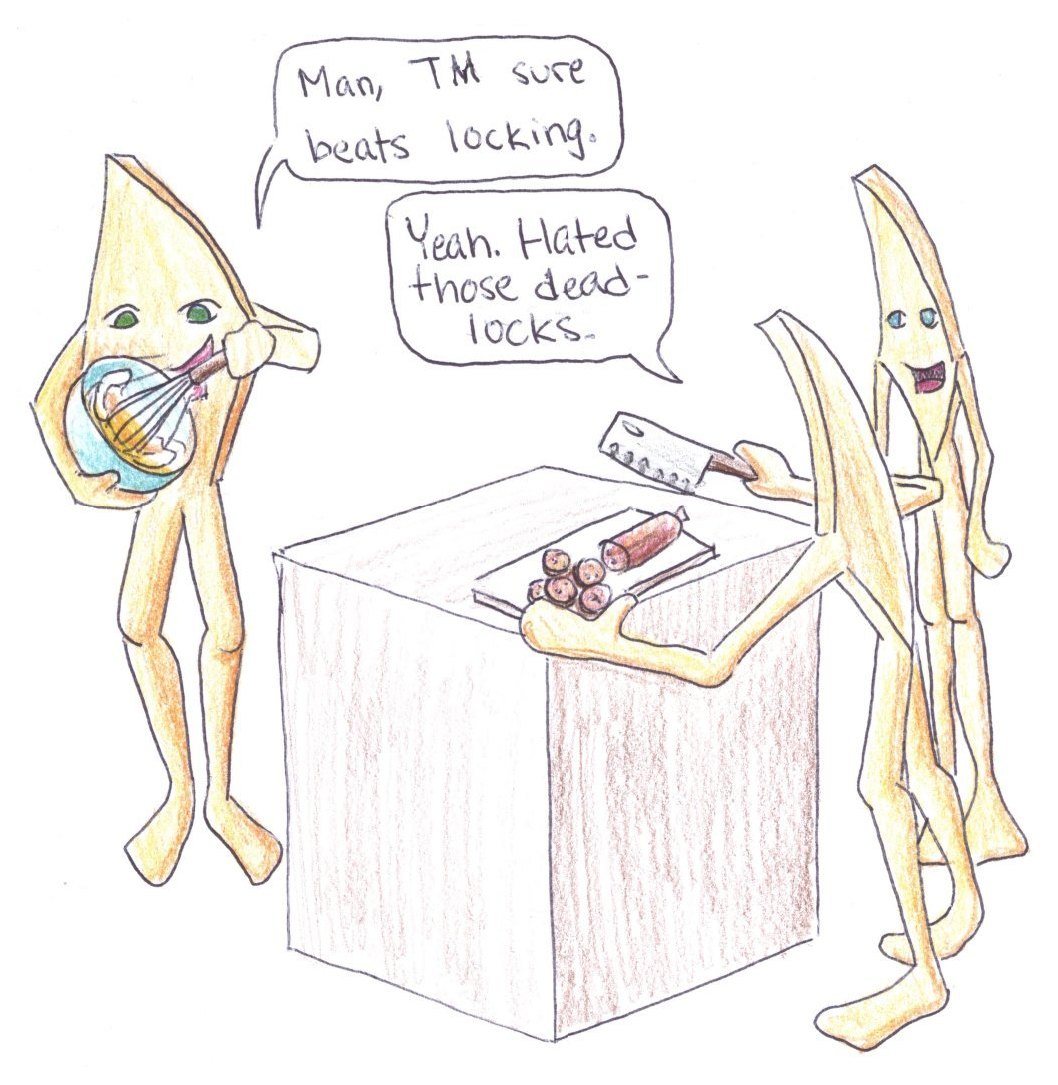
\includegraphics{cartoons/TM-the-vision}}
\caption{The STM Vision}
\ContributedBy{Figure}{fig:future:The STM Vision}{Melissa Broussard}
\end{figure}

\begin{figure}[tbp]
\centering
\resizebox{2.7in}{!}{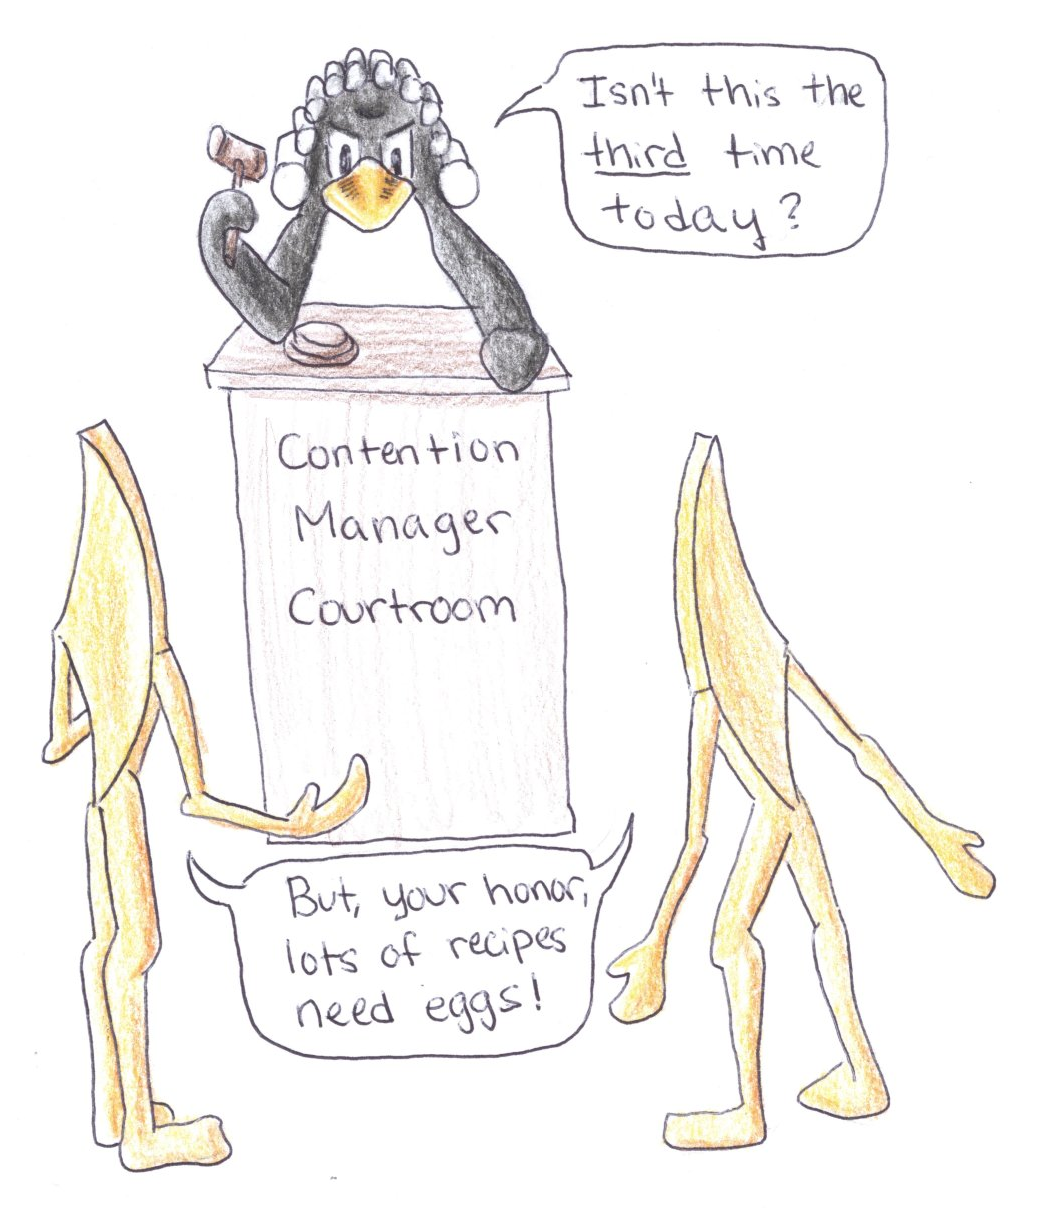
\includegraphics{cartoons/TM-the-reality-conflict}}
\caption{The STM Reality: Conflicts}
\ContributedBy{Figure}{fig:future:The STM Reality: Conflicts}{Melissa Broussard}
\end{figure}

\begin{figure}[tbp]
\centering
\resizebox{3in}{!}{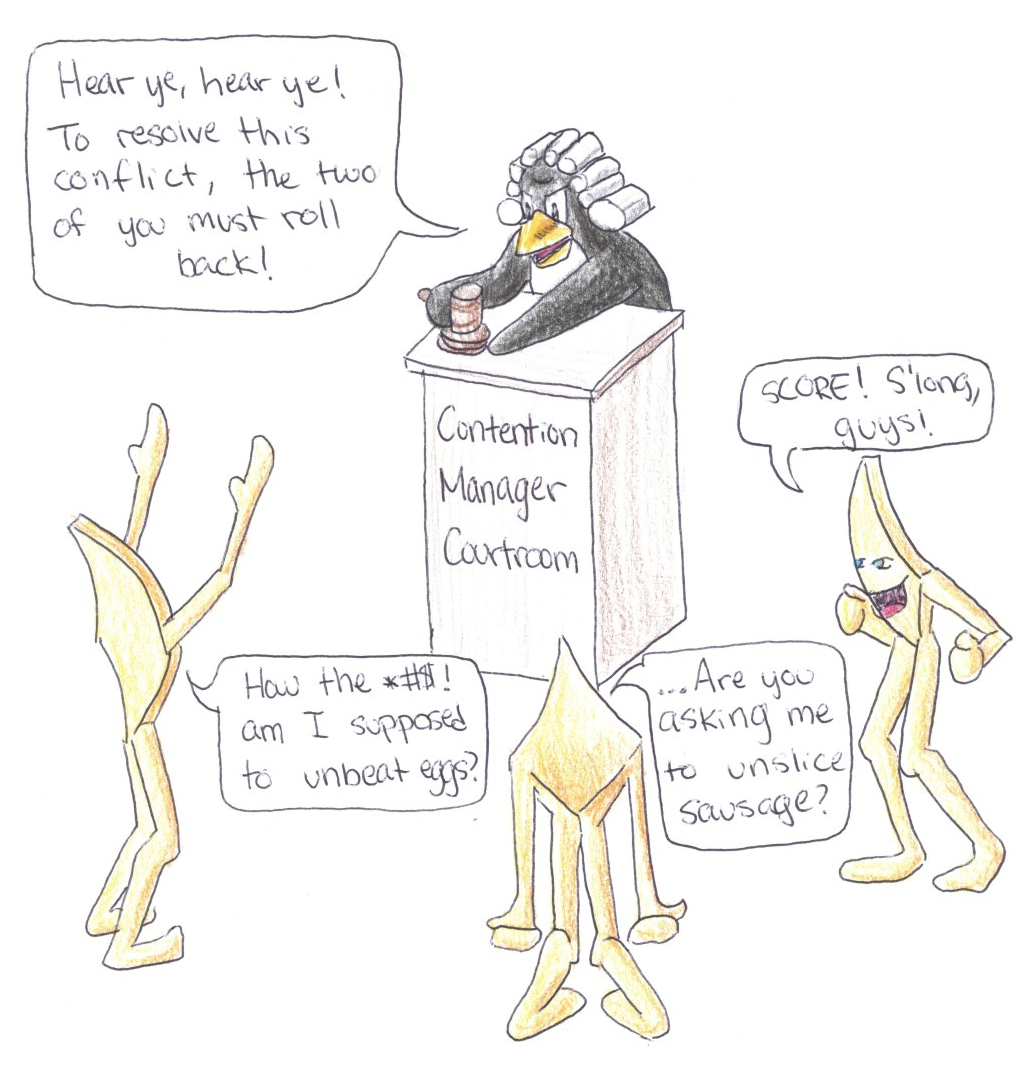
\includegraphics{cartoons/TM-the-reality-nonidempotent}}
\caption{The STM Reality: Irrevocable Operations}
\ContributedBy{Figure}{fig:future:The STM Reality: Irrevocable Operations}{Melissa Broussard}
\end{figure}

\begin{figure}[tbp]
\centering
\resizebox{2.7in}{!}{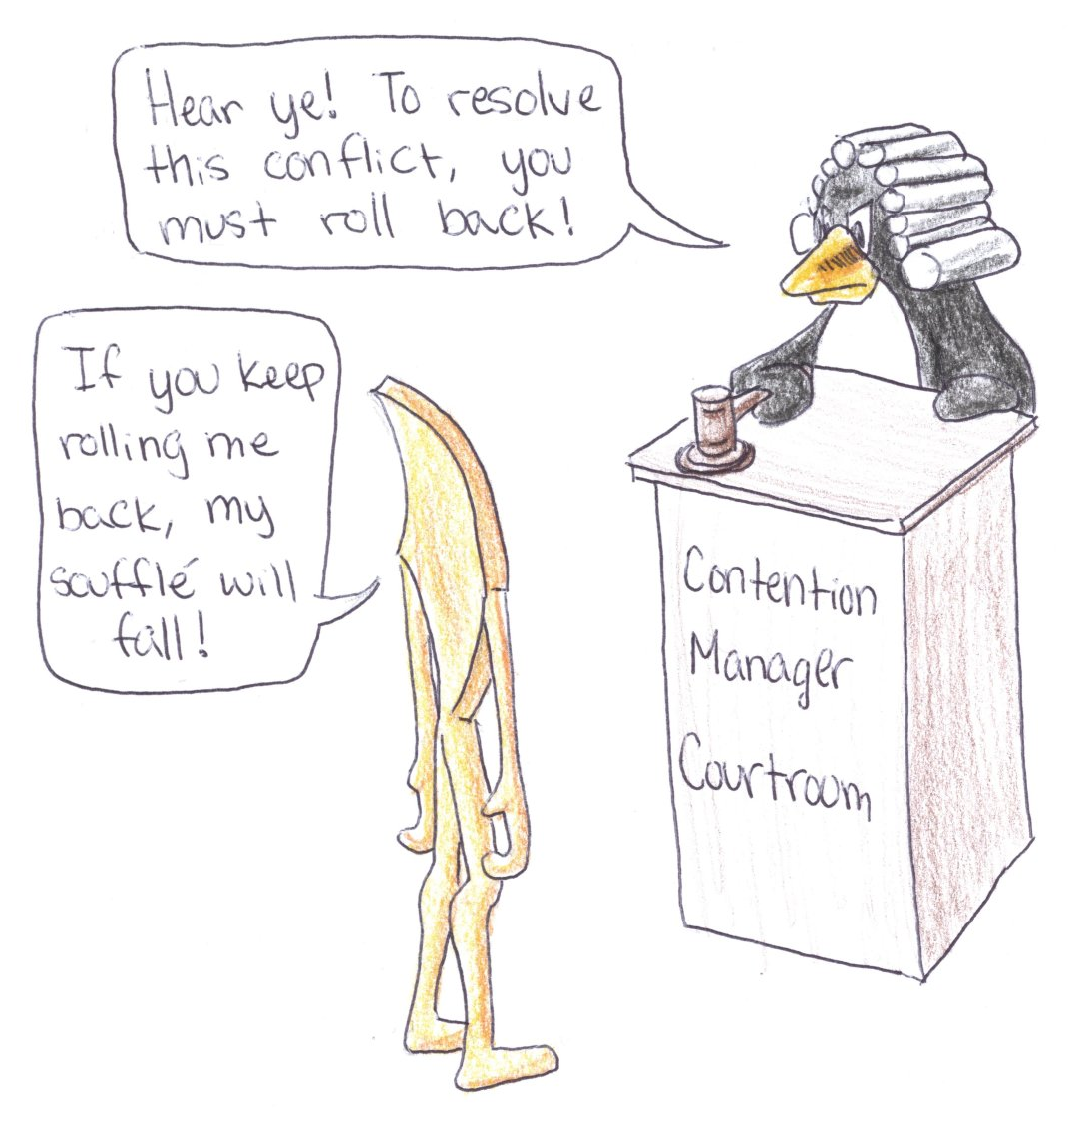
\includegraphics{cartoons/TM-the-reality-realtime}}
\caption{The STM Reality: Realtime Response}
\ContributedBy{Figure}{fig:future:The STM Reality: Realtime Response}{Melissa Broussard}
\end{figure}

But for the moment, the current state of STM
can best be summarized with a series of cartoons.
First,
\cref{fig:future:The STM Vision}
shows the STM vision.
As always, the reality is a bit more nuanced, as fancifully depicted by
\cref{fig:future:The STM Reality: Conflicts,%
fig:future:The STM Reality: Irrevocable Operations,%
fig:future:The STM Reality: Realtime Response}.\footnote{
	Recent academic work-in-progress has investigated lock-based STM
	systems for real-time use~\cite{JimAnderson2019STMRT,CatherineNemitz2018LockSTMrealtime},
	albeit without any performance results, and with some indications
	that real-time hybrid STM/HTM systems must choose between fast
	common-case performance and worst-case forward-progress
	guarantees~\cite{DBLP:journals/corr/AlistarhKKRS14,MartinSchoeberl2010realtimeTM}.}
Less fanciful STM retrospectives are also
available~\cite{JoeDuffy2010RetroTM,JoeDuffy2010RetroTM2}.

Some commercially available hardware supports restricted variants of
HTM, which are addressed in the following section.
